\documentclass[preprint,12pt]{elsarticle}
%DIF LATEXDIFF DIFFERENCE FILE
%DIF DEL /tmp/mk/old_flat.tex   Thu Oct  1 18:40:06 2026
%DIF ADD /tmp/mk/new_flat.tex   Thu Oct  1 18:40:07 2026





\usepackage{amssymb}
\usepackage{amsmath}
\usepackage{color,array}
\usepackage{xcolor}
\usepackage{graphicx}
\usepackage{algorithm}
\usepackage{amsmath,amsfonts}
\usepackage{array}
\usepackage{pgfplots}
\usepackage{amsmath} \newcommand{\StopGradient}[1]{\text{StopGradient}(#1)}
\pgfplotsset{compat=1.17}
\usepackage{textcomp}
\usepackage{url}
\usepackage{xcolor}
\usepackage{verbatim}
\usepackage{graphicx}
\usepackage{algorithm}
\usepackage{algpseudocode}
\usepackage{tikz}
\usepackage{booktabs} 
\usepackage{subcaption} \usepackage{amsmath,amsfonts}
\usepackage{array}
\usepackage{cite}
\usepackage{tikz}
\usepackage{adjustbox}
\usepackage{amsmath}      \usepackage{amssymb}      \usepackage{amsthm}       \DeclareMathOperator*{\argmin}{argmin}
\DeclareMathOperator*{\argmax}{argmax} \newtheorem{thm}{Theorem}
\newtheorem{lem}[thm]{Lemma} \newtheorem{defn}{Definition}[section] \newtheorem{theorem}{Theorem}[section]
\newtheorem{lemma}[theorem]{Lemma}
\newtheorem{corollary}[theorem]{Corollary}
\newtheorem{proposition}[theorem]{Proposition}
\newtheorem{definition}{Definition}[section]
\newtheorem{assumption}{Assumption}[section]
\newtheorem{remark}{Remark}[section]
\usepackage{amsmath} 

\usetikzlibrary{
    arrows.meta,
    positioning,
    shapes.geometric,
    matrix,
    calc,
    fit}
\usepackage{natbib}
\usepackage{textcomp}
\usepackage{url}
\usepackage{verbatim}
\usepackage{graphicx}
\usepackage{algorithm}
\usepackage{algpseudocode}
\usepackage{tikz}
\usepackage{booktabs} 




\journal{Nuclear Physics B}
%DIF PREAMBLE EXTENSION ADDED BY LATEXDIFF
%DIF CFONT PREAMBLE %DIF PREAMBLE
\RequirePackage{color}\definecolor{RED}{rgb}{1,0,0}\definecolor{BLUE}{rgb}{0,0,1} %DIF PREAMBLE
\DeclareOldFontCommand{\sf}{\normalfont\sffamily}{\mathsf} %DIF PREAMBLE
\providecommand{\DIFadd}[1]{{\protect\color{blue} \sf #1}} %DIF PREAMBLE
\providecommand{\DIFdel}[1]{{\protect\color{red} \scriptsize #1}} %DIF PREAMBLE
%DIF SAFE PREAMBLE %DIF PREAMBLE
\providecommand{\DIFaddbegin}{} %DIF PREAMBLE
\providecommand{\DIFaddend}{} %DIF PREAMBLE
\providecommand{\DIFdelbegin}{} %DIF PREAMBLE
\providecommand{\DIFdelend}{} %DIF PREAMBLE
\providecommand{\DIFmodbegin}{} %DIF PREAMBLE
\providecommand{\DIFmodend}{} %DIF PREAMBLE
%DIF FLOATSAFE PREAMBLE %DIF PREAMBLE
\providecommand{\DIFaddFL}[1]{\DIFadd{#1}} %DIF PREAMBLE
\providecommand{\DIFdelFL}[1]{\DIFdel{#1}} %DIF PREAMBLE
\providecommand{\DIFaddbeginFL}{} %DIF PREAMBLE
\providecommand{\DIFaddendFL}{} %DIF PREAMBLE
\providecommand{\DIFdelbeginFL}{} %DIF PREAMBLE
\providecommand{\DIFdelendFL}{} %DIF PREAMBLE
\newcommand{\DIFscaledelfig}{0.5}
%DIF HIGHLIGHTGRAPHICS PREAMBLE %DIF PREAMBLE
\RequirePackage{settobox} %DIF PREAMBLE
\RequirePackage{letltxmacro} %DIF PREAMBLE
\newsavebox{\DIFdelgraphicsbox} %DIF PREAMBLE
\newlength{\DIFdelgraphicswidth} %DIF PREAMBLE
\newlength{\DIFdelgraphicsheight} %DIF PREAMBLE
% store original definition of \includegraphics %DIF PREAMBLE
\LetLtxMacro{\DIFOincludegraphics}{\includegraphics} %DIF PREAMBLE
\newcommand{\DIFaddincludegraphics}[2][]{{\color{blue}\fbox{\DIFOincludegraphics[#1]{#2}}}} %DIF PREAMBLE
\newcommand{\DIFdelincludegraphics}[2][]{% %DIF PREAMBLE
\sbox{\DIFdelgraphicsbox}{\DIFOincludegraphics[#1]{#2}}% %DIF PREAMBLE
\settoboxwidth{\DIFdelgraphicswidth}{\DIFdelgraphicsbox} %DIF PREAMBLE
\settoboxtotalheight{\DIFdelgraphicsheight}{\DIFdelgraphicsbox} %DIF PREAMBLE
\scalebox{\DIFscaledelfig}{% %DIF PREAMBLE
\parbox[b]{\DIFdelgraphicswidth}{\usebox{\DIFdelgraphicsbox}\\[-\baselineskip] \rule{\DIFdelgraphicswidth}{0em}}\llap{\resizebox{\DIFdelgraphicswidth}{\DIFdelgraphicsheight}{% %DIF PREAMBLE
\setlength{\unitlength}{\DIFdelgraphicswidth}% %DIF PREAMBLE
\begin{picture}(1,1)% %DIF PREAMBLE
\thicklines\linethickness{2pt} %DIF PREAMBLE
{\color[rgb]{1,0,0}\put(0,0){\framebox(1,1){}}}% %DIF PREAMBLE
{\color[rgb]{1,0,0}\put(0,0){\line( 1,1){1}}}% %DIF PREAMBLE
{\color[rgb]{1,0,0}\put(0,1){\line(1,-1){1}}}% %DIF PREAMBLE
\end{picture}% %DIF PREAMBLE
}\hspace*{3pt}}} %DIF PREAMBLE
} %DIF PREAMBLE
\LetLtxMacro{\DIFOaddbegin}{\DIFaddbegin} %DIF PREAMBLE
\LetLtxMacro{\DIFOaddend}{\DIFaddend} %DIF PREAMBLE
\LetLtxMacro{\DIFOdelbegin}{\DIFdelbegin} %DIF PREAMBLE
\LetLtxMacro{\DIFOdelend}{\DIFdelend} %DIF PREAMBLE
\DeclareRobustCommand{\DIFaddbegin}{\DIFOaddbegin \let\includegraphics\DIFaddincludegraphics} %DIF PREAMBLE
\DeclareRobustCommand{\DIFaddend}{\DIFOaddend \let\includegraphics\DIFOincludegraphics} %DIF PREAMBLE
\DeclareRobustCommand{\DIFdelbegin}{\DIFOdelbegin \let\includegraphics\DIFdelincludegraphics} %DIF PREAMBLE
\DeclareRobustCommand{\DIFdelend}{\DIFOaddend \let\includegraphics\DIFOincludegraphics} %DIF PREAMBLE
\LetLtxMacro{\DIFOaddbeginFL}{\DIFaddbeginFL} %DIF PREAMBLE
\LetLtxMacro{\DIFOaddendFL}{\DIFaddendFL} %DIF PREAMBLE
\LetLtxMacro{\DIFOdelbeginFL}{\DIFdelbeginFL} %DIF PREAMBLE
\LetLtxMacro{\DIFOdelendFL}{\DIFdelendFL} %DIF PREAMBLE
\DeclareRobustCommand{\DIFaddbeginFL}{\DIFOaddbeginFL \let\includegraphics\DIFaddincludegraphics} %DIF PREAMBLE
\DeclareRobustCommand{\DIFaddendFL}{\DIFOaddendFL \let\includegraphics\DIFOincludegraphics} %DIF PREAMBLE
\DeclareRobustCommand{\DIFdelbeginFL}{\DIFOdelbeginFL \let\includegraphics\DIFdelincludegraphics} %DIF PREAMBLE
\DeclareRobustCommand{\DIFdelendFL}{\DIFOaddendFL \let\includegraphics\DIFOincludegraphics} %DIF PREAMBLE
%DIF COLORLISTINGS PREAMBLE %DIF PREAMBLE
\RequirePackage{listings} %DIF PREAMBLE
\RequirePackage{color} %DIF PREAMBLE
\lstdefinelanguage{DIFcode}{ %DIF PREAMBLE
%DIF DIFCODE_CFONT %DIF PREAMBLE
  moredelim=[il][\color{red}\scriptsize]{\%DIF\ <\ }, %DIF PREAMBLE
  moredelim=[il][\color{blue}\sffamily]{\%DIF\ >\ } %DIF PREAMBLE
} %DIF PREAMBLE
\lstdefinestyle{DIFverbatimstyle}{ %DIF PREAMBLE
	language=DIFcode, %DIF PREAMBLE
	basicstyle=\ttfamily, %DIF PREAMBLE
	columns=fullflexible, %DIF PREAMBLE
	keepspaces=true %DIF PREAMBLE
} %DIF PREAMBLE
\lstnewenvironment{DIFverbatim}{\lstset{style=DIFverbatimstyle}}{} %DIF PREAMBLE
\lstnewenvironment{DIFverbatim*}{\lstset{style=DIFverbatimstyle,showspaces=true}}{} %DIF PREAMBLE
%DIF END PREAMBLE EXTENSION ADDED BY LATEXDIFF

\begin{document}

\begin{frontmatter}





\title{SODA: Stabilized Optimal Transport Based Domain Alignment for Domain Generalization via a Dynamic Feature Reservoir}














            
\begin{abstract}
Learning domain-invariant representations is a fundamental challenge in Domain Generalization (DG). While Optimal Transport (OT) provides a geometrically principled framework for distribution alignment, its effectiveness in DG is limited by pivot instability, aligning to small-batch empirical distributions introduces high gradient variance, driving optimization toward spurious correlations. We introduce SODA (Stabilized Optimal Transport Domain Alignment) to address this limitation. Our key contribution is the Dynamic Feature Reservoir (DFR), a high-capacity FIFO queue that decouples the alignment target's sample size from the training batch size. The DFR serves as a stable, non-parametric pivot distribution, enabling \DIFdelbegin \DIFdel{Sinkhorn divergence computation }\DIFdelend \DIFaddbegin \DIFadd{entropic OT alignment }\DIFaddend against a statistically significant feature population. Experiments on seven DG benchmarks demonstrate that SODA achieves consistently competitive or state-of-the-art accuracy while reducing \DIFdelbegin \DIFdel{inter-run performance variance compared to OT alignment methods}\DIFdelend \DIFaddbegin \DIFadd{the variance of the alignment gradient compared to batch-derived pivots}\DIFaddend , validating the importance of pivot stability for robust domain alignment.
\end{abstract}





\begin{keyword}




Optimal Transport \sep Domain Generalization \sep Domain Alignment \sep Dynamic Feature Reservoir \sep Wasserstein Distance 
\end{keyword}

\end{frontmatter}




















































\section{Introduction}
\label{sec:introduction}

The success of deep learning in computer vision relies on the assumption that training and testing data share the same distribution. In practice, this assumption is frequently violated: models trained in one environment often fail when deployed in another due to domain shifts in factors such as lighting, viewpoint, or sensor characteristics. Domain Generalization (DG) addresses this challenge by learning models from multiple source domains that generalize robustly to unseen target domains~\citep{zhou2022domain}. Existing DG paradigms include data augmentation to synthesize diversity, meta-learning to acquire generalization strategies, and domain alignment, which explicitly learns domain-invariant feature representations.

Within the domain alignment paradigm, the goal is to minimize discrepancy between feature distributions of different source domains. Prior methods have employed statistical metrics such as Maximum Mean Discrepancy (MMD)~\citep{li2018domain_mmd} or adversarial training inspired by Domain-Adversarial Neural Networks (DANN)~\citep{ganin2016domain}. However, adversarial approaches often suffer from training instability and mode collapse, while MMD-based methods are sensitive to kernel selection and bandwidth hyperparameters. We argue that Optimal Transport (OT) offers a more principled alternative. OT provides a geometrically grounded framework for comparing probability distributions, yielding meaningful distances even when distribution supports do not overlap, which is a common scenario in DG. The Sinkhorn algorithm~\citep{cuturi2013sinkhorn} enables efficient, differentiable OT computation suitable for deep learning.

Despite its theoretical appeal, a critical limitation has hindered OT's effectiveness in multi-source DG: the instability of the alignment pivot. Aligning multiple source domains requires a common reference distribution. Conventional approaches use batch-derived targets, such as features from a randomly selected source domain or the pooled features within the current minibatch. These ephemeral pivots exhibit high variance, fluctuating substantially with each training step due to stochastic data sampling. This \textit{pivot instability} creates an unreliable optimization landscape, introducing noisy and often conflicting gradient signals that hinder convergence to domain-invariant representations.

\begin{sloppypar} 
This paper addresses this foundational challenge through SODA (\underline{S}tabilized \underline{O}ptimal Transport Based \underline{D}omain \underline{A}lignment), a framework that stabilizes OT-based alignment via a consistent target distribution. Our key contribution is the Dynamic Feature Reservoir (DFR), a high-capacity, first-in-first-out (FIFO) feature queue that serves as a non-parametric pivot distribution. The large capacity buffers the pivot from minibatch fluctuations, ensuring stability, while the FIFO update rule enables gradual adaptation as the feature extractor improves during training. This design yields a pivot that is stable over short timescales yet adaptive over long timescales. By aligning all source domains to this reservoir using a regularized OT loss, SODA provides a smooth optimization landscape for learning robust features. Extensive experiments on seven DG benchmarks, including five real-world datasets, demonstrate that SODA achieves consistently competitive or state-of-the-art accuracy with \DIFdelbegin \DIFdel{substantially reduced performance variance across runs}\DIFdelend \DIFaddbegin \DIFadd{a lower variance of the alignment gradient than batch-derived pivots}\DIFaddend .
\end{sloppypar} 

The DFR design draws inspiration from memory queues in self-supervised learning (MoCo~\citep{he2020momentum}) and semi-supervised learning (Mean Teacher~\citep{tarvainen2017mean}). However, the DFR serves a fundamentally different mathematical role: rather than providing negative samples for contrastive learning or enforcing temporal consistency through parameter averaging, the DFR acts as a Monte Carlo estimator for the target distribution in Wasserstein space. This enables computing transport plans against a sample size $K$ that is substantially larger than the mini-batch size $B$, addressing the sample complexity limitations inherent in high-dimensional distribution matching~\citep{dong2020how}. A detailed comparison of these mechanisms is provided in Section~\ref{sec:stability_mechanisms}.

Our main contributions are:
\begin{itemize}
    \item We identify that standard mini-batch OT alignment suffers from high gradient variance due to \textit{pivot instability}, where batch-derived target distributions are statistically impoverished and fluctuate across iterations.
    \item We propose the Dynamic Feature Reservoir (DFR), which decouples the alignment target's sample size ($K$) from the training batch size ($B$), enabling low-variance geometric alignment without increasing batch memory requirements.
    \item We demonstrate that stabilizing the transport target yields robust generalization, achieving consistently competitive or state-of-the-art accuracy across seven DG benchmarks while reducing \DIFdelbegin \DIFdel{inter-run variance by $3\times$ }\DIFdelend \DIFaddbegin \DIFadd{the pivot-induced variance of the alignment gradient }\DIFaddend compared to batch-derived alignment methods.
\end{itemize} \section{Related Work}
\label{sec:related_work}

This section reviews the literature on Domain Generalization (DG), situating our work within the broader research landscape. We first provide an overview of major DG paradigms, then examine domain alignment methods. We critically analyze the use of Optimal Transport for this task, identifying the pivot instability problem that motivates our work. Finally, we compare stability mechanisms across representation learning contexts to clarify the distinct role of our Dynamic Feature Reservoir.

\subsection{Major Paradigms in Domain Generalization}

The pursuit of generalizable models has given rise to several research paradigms, each with distinct strengths and limitations.

\textbf{Data Augmentation.} These methods enrich training data with samples from synthetic domains, exposing the model to a wider range of variations. Approaches range from feature-level style randomization such as MixStyle~\citep{zhou2021mixstyle} to frequency-domain perturbations~\citep{xu2021fourier}. While effective at increasing diversity, synthesized data may not accurately represent true unseen target distributions, potentially introducing artifacts that do not aid generalization.

\textbf{Disentangled Representation Learning.} These methods explicitly separate a feature vector $z$ into a domain-invariant component $z_{inv}$ and a domain-specific component $z_{spec}$, such that $z = [z_{inv}, z_{spec}]$. The domain-invariant part captures semantic content required for the primary task, while the domain-specific part captures stylistic factors unique to each domain~\citep{bui2021exploiting, peng2019domain, ilse2020diva}. While conceptually elegant, these methods require carefully designed encoder-decoder architectures and can be sensitive to hyperparameter tuning. Ensuring that semantic information does not leak into the domain-specific component remains challenging.

\textbf{Invariant Risk Minimization.} IRM~\citep{arjovsky2019invariant} formalizes DG by seeking representations under which the optimal classifier is identical across all training domains. The objective learns a feature extractor $f_\theta$ such that a single classifier $C_\psi$ is simultaneously optimal for all environments $e \in \mathcal{E}_{tr}$:
\begin{equation}
    \min_{\theta, \psi} \sum_{e \in \mathcal{E}_{tr}} R_e(C_\psi \circ f_\theta) \quad \text{subject to} \quad C_\psi \in \underset{\bar{C}_{\bar{\psi}}}{\text{argmin}} \ R_e(\bar{C}_{\bar{\psi}} \circ f_\theta) \ \forall e \in \mathcal{E}_{tr},
\end{equation}
where $R_e$ is the expected loss over environment $e$. Despite its theoretical soundness, practical optimization of IRM has proven difficult, and performance can be sensitive to training environment diversity~\citep{gulrajani2020search}.

\textbf{Meta-Learning.} These methods recast DG as learning to learn by simulating domain shift during training through virtual training and testing splits. Some approaches learn explicit regularization functions that improve generalization~\citep{balaji2018metareg}, while others meta-learn models robust to domain-specific feature statistics~\citep{dou2019meta_invariant}.

\textbf{Optimization-Based Methods.} Recent methods regularize training dynamics to promote robustness. Sharpness-Aware Minimization (SAM)~\citep{foret2021sharpness} and its DG variants such as GSAM~\citep{zhuang2022surrogate} seek parameters in flat loss landscape minima, which correlate with better generalization. Gradient matching methods enforce invariance by minimizing gradient variance or maximizing gradient similarity across domains~\citep{shi2022gradient, rame2022fishr}. Arithmetic Meta-Learning~\citep{Wang2025BalancedDF} proposes balanced gradient update directions, while Gradient-Guided Annealing~\citep{gga2025} introduces search mechanisms to escape local minima.

These optimization-based methods achieve robustness by regularizing the loss landscape or gradient properties. Our work takes a complementary approach, focusing on the geometric structure of the feature space itself. We contend that stable geometric alignment between feature manifolds provides a distinct form of invariance that can be combined with optimization-based advances. As shown in Table~\ref{tab:real_results}, stabilizing the alignment pivot yields performance competitive with or superior to complex optimization strategies.

\subsection{Domain Alignment for Invariant Representation Learning}

Domain alignment methods learn a feature extractor $f_\theta$ that maps inputs from any source domain $\mathcal{D}_i$ into a common feature space $\mathcal{Z}$, such that feature distributions $P(f_\theta(x) | x \in \mathcal{D}_i)$ become indistinguishable across domains.

\begin{sloppypar} 
\textbf{Adversarial Alignment.} Domain-Adversarial Neural Networks (DANN)~\citep{ganin2016domain} employ a minimax game between a feature extractor $f_\theta$, a task classifier $C_\psi$, and a domain discriminator $g_\phi$. The feature extractor minimizes classification loss while maximizing domain confusion through a gradient reversal layer:
\begin{equation}
    \min_{\theta, \psi} \max_{\phi} \quad \mathcal{L}_{\text{cls}}(C_\psi(f_\theta(x)), y) - \lambda \mathcal{L}_{\text{adv}}(g_\phi(f_\theta(x)), d).
\end{equation}
While powerful, this adversarial dynamic often leads to unstable training and mode collapse, making it challenging to tune effectively.
\end{sloppypar} 

\textbf{Statistical Discrepancy Minimization.} Maximum Mean Discrepancy (MMD)~\citep{gretton2012kernel, li2018domain_mmd} measures the distance between mean embeddings of domain distributions in a Reproducing Kernel Hilbert Space (RKHS):
\begin{equation}
    \mathcal{L}_{\text{MMD}}^2(\mathcal{D}_i, \mathcal{D}_j) = \left\| \mathbb{E}_{x_i \sim \mathcal{D}_i}[\phi(f_\theta(x_i))] - \mathbb{E}_{x_j \sim \mathcal{D}_j}[\phi(f_\theta(x_j))] \right\|_{\mathcal{H}}^2,
\end{equation}
where $\phi(\cdot)$ is the feature map to RKHS $\mathcal{H}$ induced by a chosen kernel. The effectiveness of MMD-based methods depends critically on kernel selection and hyperparameters, which can limit practical performance.

\textbf{Other Approaches.} Additional paradigms include probabilistic methods that learn domain density transformations to map source densities to a shared latent density~\citep{gong2016domain}, and knowledge distillation approaches where a student model learns domain-invariant representations by mimicking a robust pre-trained teacher~\citep{niu2024knowledge}. These methods tackle DG through probabilistic or information-theoretic perspectives. Our work complements this literature by pursuing a geometric perspective, arguing that directly aligning feature manifolds via geometric distance offers a more direct mechanism when distributions are complex and non-overlapping.

\subsection{Optimal Transport for Domain Generalization}

The limitations of statistical metrics have motivated adopting Optimal Transport (OT) as a geometric alternative for distribution alignment. First formalized by Monge and relaxed by Kantorovich, OT theory provides a principled framework for comparing probability measures~\citep{villani2009optimal}. For distributions $\mu$ and $\nu$, the $p$-Wasserstein distance is the cost of the optimal transport plan transforming $\mu$ into $\nu$:
\begin{equation}
    W_p(\mu, \nu) = \left( \inf_{\pi \in \Pi(\mu, \nu)} \int_{\mathcal{Z} \times \mathcal{Z}} \underbrace{c(z_1, z_2)^p}_{\text{Cost per unit}} \cdot \underbrace{d\pi(z_1, z_2)}_{\text{Mass moved}} \right)^{1/p},
\end{equation}
where $\Pi(\mu, \nu)$ is the set of valid transport plans with marginals $\mu$ and $\nu$, and $c(z_1, z_2)$ is typically the Euclidean distance. A key advantage of Wasserstein distance is its ability to compare distributions even when their supports do not overlap, where metrics like MMD may fail. While direct computation is prohibitive, entropic regularization solved via the Sinkhorn algorithm~\citep{cuturi2013sinkhorn} provides a fast, differentiable approximation suitable for deep learning~\citep{peyre2019computational}.

Several works have applied OT to DG, validating its potential without addressing pivot stability. HFedATM~\citep{wang2021hfedatm} uses OT in federated DG but relies on regularized mean aggregation of client models, which still constitutes a batch-dependent, low-capacity target. Zhou et al.~\citep{zhou2021domain} combine OT with metric similarity learning, but alignment is performed pairwise between domains or against batch-derived targets, inheriting potential instability. Works exploring OT for distributional robustness~\citep{gao2023optimal} focus on theoretical robustness guarantees rather than practical challenges of creating stable targets for multi-source DG. These works validate OT's potential but do not address the unstable optimization caused by fluctuating alignment targets. This \textit{pivot instability} represents a fundamental barrier to effectively leveraging OT for domain generalization, which our work directly addresses.

\subsection{Stability Mechanisms in Representation Learning}
\label{sec:stability_mechanisms}

Our Dynamic Feature Reservoir draws inspiration from momentum and memory mechanisms that create stability in other representation learning contexts. However, as we detail below, the DFR serves a fundamentally different mathematical role.

\textbf{Mean Teacher}~\citep{tarvainen2017mean} improves semi-supervised learning by maintaining a momentum-updated teacher model that provides consistent pseudo-labels for unlabeled data, creating stability in \textit{parameter space}.

\textbf{Momentum Contrast (MoCo)}~\citep{he2020momentum} uses a FIFO queue of feature vectors as a large, stable set of negative samples for \textit{contrastive learning} in self-supervised settings.
\begin{sloppypar} 
\textbf{SODA (Ours)} employs the Dynamic Feature Reservoir as a \textit{non-parametric density estimator} for the target distribution in Wasserstein space, enabling geometric alignment against a high-capacity pivot.
\end{sloppypar} 
Table~\ref{tab:queue_comparison} summarizes the key distinctions between these mechanisms.

\begin{table}[t]
\caption{Comparison of memory queue mechanisms across learning paradigms. The DFR serves a fundamentally different mathematical role as a distributional target for geometric alignment rather than a source of contrastive negatives or parameter averaging.}
\begin{adjustbox}{width=1.0\textwidth}

\label{tab:queue_comparison}
\centering
\small
\begin{tabular}{lccc}
\toprule
\textbf{Aspect} & \textbf{MoCo} & \textbf{Mean Teacher} & \textbf{SODA (Ours)} \\
\midrule
Memory contents & Features & Parameters & Features \\
Memory purpose & Negative samples & Pseudo-labels & Distribution estimate \\
Loss function & InfoNCE (contrastive) & Consistency & Sinkhorn (geometric) \\
Mathematical role & Softmax denominator & Teacher network & Monte Carlo estimator \\
Stability target & Instance discrimination & Label consistency & Transport plan \\
Requires momentum encoder & Yes & Yes & No \\
\bottomrule
\end{tabular}
\end{adjustbox}
\end{table}

The critical distinction lies in mathematical role. In MoCo, the queue provides negative samples to stabilize the InfoNCE loss denominator for instance discrimination. In Mean Teacher, momentum is applied to network parameters to generate stable pseudo-labels. In SODA, the queue serves as a Monte Carlo estimator for the target distribution in Wasserstein space. This enables computing transport plans against a sample size $K$ substantially larger than the mini-batch size $B$, circumventing the sample complexity limitations inherent in high-dimensional distribution matching~\citep{dong2020how}. The queue does not participate in any contrastive or consistency objective; it defines the geometric alignment target itself. To our knowledge, SODA is the first framework to employ a memory queue specifically to create a stable, non-parametric distributional target for geometric domain alignment. \section{Methodology}
\label{sec:methodology}
\usetikzlibrary{
    arrows.meta,
    backgrounds,
    calc,
    matrix,
    positioning,
    shapes.geometric
}

\definecolor{bggray}{HTML}{f8f9fa}
\definecolor{darkblue}{HTML}{2c3e50}
\definecolor{lightbluefill}{HTML}{e3f2fd}
\definecolor{blueborder}{HTML}{1976d2}
\definecolor{lightgreenfill}{HTML}{e8f5e8}
\definecolor{greenborder}{HTML}{388e3c}
\definecolor{lightorangefill}{HTML}{fff3e0}
\definecolor{orangeborder}{HTML}{f57c00}
\definecolor{lightpurplefill}{HTML}{f3e5f5}
\definecolor{purpleborder}{HTML}{7b1fa2}
\definecolor{featureorangeborder}{HTML}{ff8f00}
\definecolor{featureorangefill}{HTML}{fff8e1}
\definecolor{redborder}{HTML}{d32f2f}
\definecolor{lightredfill}{HTML}{ffebee}
\definecolor{deeppurpleborder}{HTML}{4527a0}
\definecolor{dfrbluefill}{HTML}{e1f5fe}
\definecolor{dfrblueborder}{HTML}{0277bd}
\definecolor{backproppink}{HTML}{e91e63}
\definecolor{legendgray}{HTML}{cccccc}
\definecolor{keygray}{HTML}{666666}
\definecolor{lightgrey}{HTML}{D3D3D3}
\definecolor{lightergrey}{HTML}{F5F5F5}

\begin{figure*}[ht]
    \centering
\resizebox{0.9\linewidth}{!}{

\begin{tikzpicture}[
    font=\sffamily,
    thick,
    node distance=20mm and 25mm,
    arrowstyle/.style={-{Stealth[length=3mm, width=2.5mm]}, line width=1.8pt},
]

\definecolor{extractorfill}{HTML}{EFEFEF}
\definecolor{blockborder}{HTML}{404040}
\definecolor{classcolor}{HTML}{B3D9FF}
\definecolor{aligncolor}{HTML}{E1D5E7}
\definecolor{lossborder}{HTML}{4472C4}
\definecolor{dfrborder}{HTML}{6A8EAE}
\definecolor{totalfill}{HTML}{FFFFFF}
\definecolor{arrowmain}{HTML}{FFC000}
\definecolor{arrowclass}{HTML}{0070C0}
\definecolor{arrowalign}{HTML}{9A009A}
\definecolor{backproppink}{HTML}{E91E63}
\definecolor{z_cell_blue}{HTML}{BDE1FB}
\definecolor{z_cell_yellow}{HTML}{FFE699}
\definecolor{dfr_item_blue}{HTML}{BDE1FB}
\definecolor{dfr_item_pink}{HTML}{E1D5E7}
\definecolor{dfr_item_yellow}{HTML}{FFE699}
\definecolor{dfr_item_green}{HTML}{C6F9C6}
\definecolor{dfr_item_red}{HTML}{F9C6C6}
\tikzset{
    inputbox/.style={rectangle, rounded corners=5pt, draw=blockborder, fill=extractorfill,minimum width=80, minimum height=40, align=center, font=\bfseries\Large},
    extractor/.style={trapezium, shape border rotate=270, trapezium left angle=70, trapezium right angle=70,
                      draw=blockborder, fill=extractorfill, minimum height=160, minimum width=60,
                      align=center, font=\bfseries\Large, line width=2.2pt},
    triangle_block/.style={isosceles triangle, shape border rotate=0, draw=blockborder,
                           minimum height=160, minimum width=100, align=center, font=\bfseries\Large},
    circle_block/.style={circle, draw=blockborder, fill=aligncolor,
                         minimum size=30mm, align=center, font=\bfseries\Large},
    lossbox/.style={rectangle, rounded corners=5pt, draw=lossborder, line width=1pt, dashed,
                    align=center, text=black, minimum height=70,
                    minimum width=70, 
                    fill=lightergrey},
    totalbox/.style={rectangle, rounded corners=8pt, draw=blockborder, fill=totalfill,minimum width=100, minimum height=50, align=center, line width=1.5pt},
    feature_vector/.style={matrix of nodes, nodes in empty cells,
                           row sep=1pt,
                           nodes={rectangle, minimum width=22pt, minimum height=10pt, draw=gray, line width=0.5pt}},
    dfr_cell/.style={rectangle, draw=dfrborder, minimum width=50mm, minimum height=6mm},
    dfr_cell_empty/.style={rectangle, draw=dfrborder, dashed, minimum width=50mm, minimum height=6mm},
}



\node[rectangle, rounded corners=5pt, draw=red, line width=1.5pt,label={[font=\bfseries\Large]left:Domain 1}] (d1) at (0, 0) {\includegraphics[width=2.5cm]{fig/giraffe_cartoon.png}};
\node[rectangle, rounded corners=5pt, draw=green, line width=1.5pt, below=5mm of d1,label={[font=\bfseries\Large]left:Domain 2}] (d2) {\includegraphics[width=2.5cm]{fig/giraffe_real.jpg}};
\node[font=\bfseries\Large] at ($(d2.south)!0!(d2.south)+(0,-1.5mm)$) {$\vdots$};
\node[rectangle, rounded corners=5pt, draw=blue, line width=1.5pt, below=5mm of d2,label={[font=\bfseries\Large]left:Domain N}] (d3) {\includegraphics[width=2.5cm]{fig/giraffe_watercolor.png}};


\node[extractor, right=25mm of d2] (fe) {Feature \\ Extractor \\ ($F_\theta$)};
\matrix (z) [feature_vector, right=10mm of fe] {
    |[fill=z_cell_blue]| \\ |[fill=z_cell_yellow]| \\ |[fill=z_cell_blue]| \\
    |[fill=z_cell_blue]| \\ |[fill=z_cell_yellow]| \\ |[fill=z_cell_blue]| \\
    |[fill=z_cell_blue]| \\ |[fill=z_cell_yellow]| \\ |[fill=z_cell_blue]| \\ 
    |[fill=z_cell_blue]| \\  
};

\node[triangle_block, fill=classcolor, right=of z, yshift=3.5cm] (classifier) {Classifier \\ ($C_\psi$)};
\node[lossbox, xshift=2cm, right=of classifier] (loss_cls) {\bfseries\large $L_{\text{cls}}$};
\node[inputbox, above=5mm of loss_cls] (labels) {Labels Y};

\node[circle_block, fill=aligncolor, right=of z, yshift=-3.5cm] (l2norm) {L2 \\ Norm};
\node[lossbox, right=of l2norm, minimum width=5.5cm, minimum height=6cm] (loss_ot) {
    \includegraphics[width=11cm]{fig/ot_loss_plot.png} \\
    \vspace{2mm}
    \bfseries\large $L_{\text{OT}}$
};

\matrix (dfr_matrix) [matrix of nodes, below=of loss_ot, row sep=1.5pt] {
    |[dfr_cell, fill=dfr_item_blue]| \\
    |[dfr_cell, fill=dfr_item_green]| \\
    |[dfr_cell, fill=dfr_item_red]| \\
    |[dfr_cell_empty]| \\
    |[dfr_cell_empty]| \\
};
\node[fit=(dfr_matrix), draw=dfrborder, line width=1.2pt, rounded corners=3pt, inner sep=3pt] (dfr) {};
\node[below=2pt of dfr, align=center] {
      \bfseries\Large Dynamic Feature Reservoir (DFR) \\ \Large $Q \in \mathbb{R}^{K \times d}$
};

\node[totalbox, right=of loss_ot, xshift=2cm, yshift=1.5cm] (loss_total) {
    \bfseries\large $L_{\text{Total}}$ \\ \mdseries\Large $= L_{\text{cls}} + \lambda L_{\text{OT}}$
};



\draw[arrowstyle, draw=black!70] (d1.east) -- (fe.west);
\draw[arrowstyle, draw=black!70] (d2.east) -- (fe.west);
\draw[arrowstyle, draw=black!70] (d3.east) -- (fe.west);
\draw[arrowstyle, draw=arrowmain] (fe.east) -- (z.west) node[midway, above, font=\bfseries\color{arrowmain}] {Z};

\coordinate (z_split_point) at ($(z.east)$);

\draw[arrowstyle, draw=arrowclass] (z_split_point) to[out=45, in=180] (classifier.west);
\draw[arrowstyle, draw=arrowalign] (z_split_point) to[out=-45, in=180] (l2norm.west);

\draw[arrowstyle, draw=arrowclass] (classifier.east) -- (loss_cls.west);
\draw[arrowstyle, draw=arrowclass] (labels.south) -- (loss_cls.north);
\draw[arrowstyle, draw=arrowalign] (l2norm.east) -- (loss_ot.west);

\draw[arrowstyle, draw=dfrborder, line width=1.5pt] (dfr.north) -- (loss_ot.south) node[midway, right, font=\small]{Read};
\draw[arrowstyle, draw=arrowalign, dashed] (l2norm.south) |- (dfr.west) node[midway, above right, font=\small]{Update};

\draw[arrowstyle, draw=black!60] (loss_cls.east) to[out=0, in=140] (loss_total.west);
\draw[arrowstyle, draw=black!60] (loss_ot.east) to[out=0, in=220] (loss_total.west);

\draw[arrowstyle, draw=backproppink, dashed] (loss_total.north) to[out=90, in=0] ($(loss_total.north) + (-6cm,10cm)$) to[out=180, in=90] ($(fe.north) + (0,1cm)$) to[out=270, in=90] (fe.north);

\begin{scope}[node distance=2mm, font=\sffamily\small, text=black,
              every node/.style={anchor=west}]
    \node[draw=black!40, fill=white, rounded corners=5pt,
          left=of dfr, xshift=-10cm, align=left] (legend_box) {
        \begin{tabular}{p{1.5cm} l}
            \tikz\draw[arrowstyle, draw=arrowclass] (0,0) -- (1,0); & Classification path \\
            \tikz\draw[arrowstyle, draw=arrowalign] (0,0) -- (1,0); & Alignment path \\
            \tikz\draw[arrowstyle, draw=arrowalign, dashed] (0,0) -- (1,0); & Update (no gradients) \\
            \tikz\draw[arrowstyle, draw=backproppink, dashed] (0,0) -- (1,0); & Backpropagation \\
            \tikz\draw[arrowstyle, draw=dfrborder] (0,0) -- (1,0); & DFR read operation \\
        \end{tabular}
    };
\end{scope}

\end{tikzpicture}
} \caption{Overview of SODA. The framework consists of a standard supervised path (\textcolor{blue}{blue}) and a stabilized OT alignment path (\textcolor{purple}{purple}). Crucially, the Dynamic Feature Reservoir (DFR) is updated via a gradient-free queue mechanism (dashed line), ensuring it acts as a stable anchor. The alignment loss $\mathcal{L}_{OT}$ minimizes the \DIFdelbeginFL \DIFdelFL{Sinkhorn divergence }\DIFdelendFL \DIFaddbeginFL \DIFaddFL{entropic OT cost }\DIFaddendFL between the current mini-batch features and the non-parametric distribution defined by the reservoir.}
\label{fig:soda_framework}    
\end{figure*} 
This section presents the SODA (\underline{S}tabilized \underline{O}ptimal Transport Based \underline{D}omain \underline{A}lignment) framework, illustrated in Figure~\ref{fig:soda_framework}. We begin with mathematical preliminaries for Domain Generalization and Optimal Transport theory. We then formally characterize the pivot instability problem and introduce our solution: the Dynamic Feature Reservoir (DFR). Finally, we present the complete SODA algorithm and analyze its computational properties.

\subsection{Problem Formulation}
\label{ssec:problem}

The objective in Domain Generalization (DG) is to learn a model that generalizes from a set of source domains to an unseen target domain. Let $\mathcal{D}_S = \{D_1, D_2, \dots, D_N\}$ be $N$ source domains, where each domain $D_i$ is characterized by a distribution $P_i(X, Y)$ over input space $\mathcal{X} \subset \mathbb{R}^d$ and label space $\mathcal{Y} = \{1, \dots, C\}$. The domain shift assumption states that marginal distributions differ across domains ($P_i(X) \neq P_j(X)$ for $i \neq j$), while the labeling function $P(Y|X)$ remains consistent. The goal is to learn a model from $\mathcal{D}_S$ that performs well on an unseen target domain $D_t$ with distribution $P_t(X, Y)$.

We decompose the model $h: \mathcal{X} \to \mathcal{Y}$ into a feature extractor $f_\theta: \mathcal{X} \to \mathcal{Z}$ mapping inputs to a latent space $\mathcal{Z} \subset \mathbb{R}^{d'}$, and a classifier $C_\psi: \mathcal{Z} \to \mathbb{R}^C$ mapping features to class logits. The expected risk on a domain with distribution $P(X,Y)$ is:
\begin{equation}
    R(f_\theta, C_\psi) := \mathbb{E}_{(x,y) \sim P(X,Y)} [\mathcal{L}(C_\psi(f_\theta(x)), y)].
\end{equation}

Since the target distribution $P_t$ is inaccessible during training, the standard approach is Empirical Risk Minimization (ERM), which minimizes average risk across source domains:
\begin{equation}
    \mathcal{L}_{\text{ERM}}(\theta, \psi) = \frac{1}{N} \sum_{i=1}^{N} \mathbb{E}_{(x,y) \sim P_i(X,Y)} [\mathcal{L}_{\text{CE}}(C_\psi(f_\theta(x)), y)],
    \label{eq:erm}
\end{equation}
where $\mathcal{L}_{\text{CE}}$ denotes Cross-Entropy loss. However, ERM may overfit to domain-specific correlations. Domain alignment methods address this by adding a regularization term $\mathcal{L}_{\text{align}}$ that penalizes discrepancies between feature distributions $P_i(Z)$ where $Z = f_\theta(X)$.

An ideal alignment objective would minimize pairwise discrepancies between all source feature distributions:
\begin{equation}
    \mathcal{L}_{\text{align-ideal}}(\theta) = \frac{1}{N(N-1)} \sum_{i \neq j} d(P_i(Z), P_j(Z)),
\end{equation}
where $d(\cdot, \cdot)$ is a discrepancy measure. This objective requires $\binom{N}{2}$ comparisons, yielding $\mathcal{O}(N^2)$ complexity per step. A tractable alternative introduces a pivot distribution $P_{\text{pivot}}$:
\begin{equation}
    \mathcal{L}_{\text{align}}(\theta) = \frac{1}{N} \sum_{i=1}^{N} d(P_i(Z), P_{\text{pivot}}),
\end{equation}
reducing complexity to $\mathcal{O}(N)$. The total training objective becomes:
\begin{equation}
    \label{eq:dg_objective}
    \mathcal{L}_{\text{Total}}(\theta, \psi) = \mathcal{L}_{\text{ERM}}(\theta, \psi) + \lambda \mathcal{L}_{\text{align}}(\theta),
\end{equation}
where $\lambda$ balances classification and alignment. The effectiveness of this strategy depends critically on (1) the discrepancy measure $d(\cdot, \cdot)$, and (2) the statistical properties of $P_{\text{pivot}}$.

\subsection{Optimal Transport Theory}
\label{ssec:ot_foundations}

\begin{figure}[t]
    \centering
    \includegraphics[width=0.8\textwidth]{fig/OT_Illustration.png}
    \caption{Optimal Transport illustration. (a) Two discrete probability measures: source $\mu$ and target $\nu$, where point size indicates mass. (b) The optimal transport plan $T^*$ describes mass flow from source to target, minimizing total transportation cost. Line thickness indicates transported mass.}
    \label{fig:ot_concept}
\end{figure}

We adopt Optimal Transport (OT) as our discrepancy measure for its geometric properties. OT finds the most efficient coupling that transforms a source measure $\mu$ into a target measure $\nu$ while minimizing transportation cost (Figure~\ref{fig:ot_concept}). Rooted in the work of Monge and Kantorovich~\citep{villani2009optimal}, OT computes the minimal effort to transform one distribution into another, which is particularly suited for comparing feature manifolds with non-overlapping supports where divergence-based measures may fail.

\subsubsection{Discrete Optimal Transport}
\begin{sloppypar} 
For discrete distributions $\mu$ and $\nu$ supported on feature vectors $\{z_1, \dots, z_m\} \subset \mathcal{Z}$ and $\{z'_1, \dots, z'_n\} \subset \mathcal{Z}$ with probability vectors $\mathbf{a} \in \Delta_m$ and $\mathbf{b} \in \Delta_n$, where the probability simplex is defined as:
\begin{equation}
    \Delta_k := \left\{ \mathbf{p} \in \mathbb{R}^k_+ \ \Big| \ \sum_{i=1}^{k} p_i = 1 \right\},
\end{equation}
we define the ground cost matrix $\mathbf{M} \in \mathbb{R}^{m \times n}$ with entries:
\DIFdelbegin \begin{displaymath}
    \DIFdel{M_{ij} = c(z_i, z'_j) = \|z_i - z'_j\|_2^2,
}\end{displaymath}%DIFAUXCMD
\DIFdelend \DIFaddbegin \begin{equation}
    \DIFadd{\label{eq:cost}
    M_{ij} = c(z_i, z'_j) = \|z_i - z'_j\|_2^2,
}\end{equation}\DIFaddend 
where we use squared Euclidean distance as the cost function.
\end{sloppypar} 
A transport plan $\mathbf{T} \in \mathbb{R}^{m \times n}_+$ specifies the mass $T_{ij}$ transported from source point $z_i$ to target point $z'_j$. Valid transport plans must satisfy marginal constraints, forming the transport polytope:
\begin{equation}
    \Pi(\mathbf{a}, \mathbf{b}) := \left\{ \mathbf{T} \in \mathbb{R}^{m \times n}_+ \ \Big| \ \mathbf{T}\mathbf{1}_n = \mathbf{a}, \ \mathbf{T}^\top\mathbf{1}_m = \mathbf{b} \right\},
\end{equation}
where $\mathbf{1}_k$ denotes the $k$-dimensional vector of ones. The constraint $\mathbf{T}\mathbf{1}_n = \mathbf{a}$ ensures mass conservation at each source point, while $\mathbf{T}^\top\mathbf{1}_m = \mathbf{b}$ ensures each target point receives its prescribed mass.

The Kantorovich formulation seeks the optimal plan minimizing total transportation cost:
\begin{equation}
    \mathcal{L}_{\mathbf{M}}(\mu, \nu) = \min_{\mathbf{T} \in \Pi(\mathbf{a}, \mathbf{b})} \langle \mathbf{T}, \mathbf{M} \rangle_F = \min_{\mathbf{T} \in \Pi(\mathbf{a}, \mathbf{b})} \sum_{i,j} T_{ij} M_{ij},
\end{equation}
where $\langle \cdot, \cdot \rangle_F$ denotes the Frobenius inner product. This linear program has complexity $\mathcal{O}(n^3 \log n)$ via network simplex algorithms, which is prohibitive for deep learning.

\subsubsection{Entropic Regularization and the Sinkhorn Algorithm}

To enable efficient computation, we adopt entropic regularization~\citep{cuturi2013sinkhorn}, which introduces a strictly convex penalty:
\begin{equation}
    \label{eq:entropic_ot}
    \mathcal{L}^\epsilon_{\mathbf{M}}(\mu, \nu) = \min_{\mathbf{T} \in \Pi(\mathbf{a}, \mathbf{b})} \langle \mathbf{T}, \mathbf{M} \rangle_F - \epsilon H(\mathbf{T}),
\end{equation}
where $\epsilon > 0$ is the regularization strength and $H(\mathbf{T})$ is the entropy of the transport plan:
\begin{equation}
    H(\mathbf{T}) = -\sum_{i,j} T_{ij}(\log T_{ij} - 1).
\end{equation}

To derive the solution, we form the Lagrangian with dual variables $\boldsymbol{\alpha} \in \mathbb{R}^m$ and $\boldsymbol{\beta} \in \mathbb{R}^n$ for the marginal constraints:
\begin{equation}
    \mathcal{L}(\mathbf{T}, \boldsymbol{\alpha}, \boldsymbol{\beta}) = \langle \mathbf{T}, \mathbf{M} \rangle_F - \epsilon H(\mathbf{T}) - \langle \boldsymbol{\alpha}, \mathbf{T}\mathbf{1}_n - \mathbf{a} \rangle - \langle \boldsymbol{\beta}, \mathbf{T}^\top\mathbf{1}_m - \mathbf{b} \rangle.
\end{equation}

Setting $\frac{\partial \mathcal{L}}{\partial T_{ij}} = 0$ yields the first-order optimality condition:
\begin{equation}
    M_{ij} + \epsilon \log T^*_{ij} - \alpha_i - \beta_j = 0,
\end{equation}
which gives the optimal transport plan in closed form:
\begin{equation}
    \label{eq:optimal_plan_form}
    T^*_{ij} = \exp\left(\frac{\alpha_i + \beta_j - M_{ij}}{\epsilon}\right) = \exp\left(\frac{\alpha_i}{\epsilon}\right) \exp\left(\frac{-M_{ij}}{\epsilon}\right) \exp\left(\frac{\beta_j}{\epsilon}\right).
\end{equation}

Defining scaling vectors $\mathbf{u} = e^{\boldsymbol{\alpha}/\epsilon} \in \mathbb{R}^m_+$ and $\mathbf{v} = e^{\boldsymbol{\beta}/\epsilon} \in \mathbb{R}^n_+$, and the Gibbs kernel $\mathbf{K} = e^{-\mathbf{M}/\epsilon}$ with entries $K_{ij} = e^{-M_{ij}/\epsilon}$, we obtain the matrix factorization:
\begin{equation}
    \mathbf{T}^*_\epsilon = \text{diag}(\mathbf{u}) \, \mathbf{K} \, \text{diag}(\mathbf{v}).
\end{equation}

The scaling vectors are determined by the marginal constraints. Substituting into $\mathbf{T}\mathbf{1}_n = \mathbf{a}$ and $\mathbf{T}^\top\mathbf{1}_m = \mathbf{b}$ yields the Sinkhorn-Knopp fixed-point equations:
\begin{equation}
    \mathbf{u} = \frac{\mathbf{a}}{\mathbf{K}\mathbf{v}}, \quad \mathbf{v} = \frac{\mathbf{b}}{\mathbf{K}^\top\mathbf{u}},
\end{equation}
where division is element-wise. Starting from $\mathbf{v}^{(0)} = \mathbf{1}_n$, the algorithm iterates:
\begin{equation}
    \mathbf{u}^{(l+1)} = \frac{\mathbf{a}}{\mathbf{K}\mathbf{v}^{(l)}}, \quad \mathbf{v}^{(l+1)} = \frac{\mathbf{b}}{\mathbf{K}^\top\mathbf{u}^{(l+1)}}.
\end{equation}

This algorithm converges linearly with rate dependent on $\epsilon$~\citep{peyre2019computational}. \DIFdelbegin \DIFdel{The resulting Sinkhorn divergence }\DIFdelend \DIFaddbegin \DIFadd{We denote the resulting \emph{entropic OT cost} by }\DIFaddend $W_\epsilon(\mu, \nu) := \mathcal{L}^\epsilon_{\mathbf{M}}(\mu, \nu)$\DIFaddbegin \DIFadd{; it }\DIFaddend is differentiable with respect to input feature locations, enabling end-to-end training. \DIFaddbegin \DIFadd{$W_\epsilon$ differs from the (debiased) Sinkhorn divergence $S_\epsilon(\mu,\nu)=W_\epsilon(\mu,\nu)-\tfrac12W_\epsilon(\mu,\mu)-\tfrac12W_\epsilon(\nu,\nu)$~\citep{feydy2019interpolating}, which removes the entropic bias so that $S_\epsilon(\mu,\mu)=0$. SODA minimizes $W_\epsilon$: our implementation uses GeomLoss~\citep{feydy2019interpolating} with \texttt{debias=False}, ground cost $\tfrac12\|x-y\|^2$ and $\epsilon=\texttt{blur}^2$, which yields the same transport plans as Eq.~(\ref{eq:entropic_ot}) with $\epsilon=2\,\texttt{blur}^2$ and half its value. Replacing $W_\epsilon$ by $S_\epsilon$ does not change accuracy in our experiments (70.8\% with either loss on OfficeHome over three seeds).
}\DIFaddend 

\subsubsection{Gradient Flow and Feature Learning}

A key property for our application is how \DIFdelbegin \DIFdel{the Sinkhorn divergence }\DIFdelend \DIFaddbegin \DIFadd{$W_\epsilon$ }\DIFaddend induces gradients on feature representations. \DIFdelbegin \DIFdel{For a }\DIFdelend \DIFaddbegin \DIFadd{The transport polytope $\Pi(\mathbf a,\mathbf b)$ does not depend on the support points and the entropic problem has a unique solution $\mathbf T^*_\epsilon$, so by the envelope theorem the gradient with respect to a }\DIFaddend source feature $z_i$, \DIFdelbegin \DIFdel{the gradient of the transport cost takes the form~\citep{peyre2019computational}:
}\begin{displaymath}
    \DIFdel{\label{eq:wasserstein_gradient}
    \nabla_{z_i} W_\epsilon(\mu, \nu) = \frac{2}{\epsilon} \sum_{j=1}^{n} T^*_{ij} (z_i - z'_j).
}\end{displaymath}%DIFAUXCMD
\DIFdelend \DIFaddbegin \DIFadd{for the squared Euclidean cost of Eq.~(\ref{eq:cost}), is~\citep{peyre2019computational}:
}\begin{equation}
    \DIFadd{\label{eq:wasserstein_gradient}
    \nabla_{z_i} W_\epsilon(\mu, \nu) = 2 \sum_{j=1}^{n} T^*_{ij} (z_i - z'_j) = 2a_i\big(z_i-\hat z_i\big),\qquad \hat z_i:=\frac{1}{a_i}\sum_{j=1}^n T^*_{ij}z'_j .
}\end{equation}\DIFaddend 

This gradient \DIFdelbegin \DIFdel{is }\DIFdelend \DIFaddbegin \DIFadd{pulls $z_i$ toward $\hat z_i$, }\DIFaddend a weighted average of \DIFdelbegin \DIFdel{directions toward target points , where weights $T^*_{ij}$ are determined by the optimal }\DIFdelend \DIFaddbegin \DIFadd{the target points matched to it, with weights given by the }\DIFaddend transport plan. Minimizing $W_\epsilon$ thus moves source features toward their optimal correspondences in the target distribution. \DIFdelbegin \DIFdel{The regularization parameter }\DIFdelend \DIFaddbegin \DIFadd{There is no explicit $1/\epsilon$ factor: }\DIFaddend $\epsilon$ \DIFdelbegin \DIFdel{controls gradient magnitude: smaller }\DIFdelend \DIFaddbegin \DIFadd{acts only through $\mathbf T^*_\epsilon$. Smaller }\DIFaddend $\epsilon$ \DIFdelbegin \DIFdel{yields larger gradients concentrated on nearest neighbors, while }\DIFdelend \DIFaddbegin \DIFadd{concentrates each row of the plan on a few nearby target points, so the gradient depends on individual target samples; }\DIFaddend larger $\epsilon$ \DIFdelbegin \DIFdel{produces smaller, more diffuse gradients. }\DIFdelend \DIFaddbegin \DIFadd{spreads it over many, and as $\epsilon\to\infty$ the plan tends to $\mathbf a\mathbf b^\top$ and the gradient only matches means. For unit-norm features the gradient norm is at most $4a_i$ for every $\epsilon$.
}\DIFaddend 

\subsubsection{Effect of Entropic Regularization on Transport Plans}

The parameter $\epsilon$ fundamentally affects the structure of $\mathbf{T}^*_\epsilon$:

\begin{proposition}[Transport Plan Entropy]
\label{prop:entropy}
As $\epsilon \to 0$, the optimal plan $\mathbf{T}^*_\epsilon$ converges to the sparse solution of the unregularized problem, approaching a permutation matrix for equal-mass distributions. As $\epsilon \to \infty$, $\mathbf{T}^*_\epsilon \to \mathbf{a}\mathbf{b}^\top$, the maximum-entropy independent coupling.
\end{proposition}

This has important implications for domain alignment:
\begin{itemize}
    \item \textbf{Low $\epsilon$}: Sparse plans create hard assignments between source and target features. Gradients are dominated by nearest-neighbor correspondences, making optimization sensitive to outliers and local density variations.
    \item \textbf{High $\epsilon$}: Dense plans distribute mass broadly, creating soft many-to-many alignments. Each source feature receives gradient contributions from multiple target features, providing implicit regularization against overfitting to specific target samples.
\end{itemize}

\DIFdelbegin \DIFdel{For domain alignment with a reservoir containing temporally heterogeneous features , higher $\epsilon$ is beneficial as it prevents overfitting to potentially stale or outlier reservoir entries (see Section~\ref{sec:experiments} for empirical validation) }\DIFdelend \DIFaddbegin \DIFadd{The reservoir contains features encoded by earlier parameters; Section~\ref{ssec:dfr} bounds the resulting bias (Proposition~\ref{prop:staleness}) and Section~\ref{sec:stability_analysis} measures it during training}\DIFaddend .

\subsection{The Pivot Instability Problem}
\label{ssec:pivot_instability}

Applying OT to multi-source DG requires a pivot distribution $P_{\text{pivot}}$ for alignment. Conventional approaches construct this pivot from the current minibatch, either using a randomly selected source domain's features or pooling all minibatch features: $P_{\text{pivot}} = \text{Uniform}(\{z_k\}_{k=1}^{B})$. Both strategies suffer from \textit{pivot instability}: the target distribution fluctuates substantially across iterations due to stochastic sampling.

\subsubsection{Formal Definition of Stability}

We formally characterize pivot stability in terms of the divergence between consecutive pivot distributions:

\begin{definition}[Pivot Stability]
\label{def:stability}
Let $P_{\text{pivot}}^{(t)}$ denote the pivot distribution at training iteration $t$. The \textit{pivot instability} $\mathcal{S}$ is the expected Wasserstein distance between consecutive pivots:
\begin{equation}
    \mathcal{S} := \mathbb{E}_t\left[W_2\left(P_{\text{pivot}}^{(t)}, P_{\text{pivot}}^{(t+1)}\right)\right].
\end{equation}
A pivot mechanism with lower $\mathcal{S}$ provides more consistent optimization targets.
\end{definition}

For batch-derived pivots reconstructed entirely each iteration, $\mathcal{S}$ equals the expected Wasserstein distance between independent samples from the feature distribution—which can be substantial in high-dimensional spaces.

\subsubsection{Impact on Gradient Variance}

Pivot instability directly affects the variance of the alignment gradient. Let $\mathbf{g}^{(t)} = \nabla_\theta \mathcal{L}_{\text{align}}^{(t)}$ denote the alignment gradient at iteration $t$. We can decompose:
\begin{equation}
    \text{Var}[\mathbf{g}^{(t)}] = \underbrace{\text{Var}[\mathbf{g}^{(t)} | P_{\text{pivot}}]}_{\text{Source sampling variance}} + \underbrace{\mathbb{E}[\text{Var}[\mathbf{g}^{(t)} | P_{\text{source}}]]}_{\text{Pivot variance}}.
\end{equation}

The first term arises from stochastic sampling of source features and is irreducible given batch size constraints. The second term arises from pivot fluctuations and can be controlled through pivot design. High pivot variance manifests as conflicting gradient directions across iterations, hindering convergence.

\subsubsection{Statistical Impossibility in High Dimensions}

The instability problem is exacerbated by a fundamental statistical limitation. \citet{dong2025distribution} establish an impossibility result for distribution matching from small samples:

\begin{theorem}[Informal, from \citet{dong2025distribution}]
\label{thm:impossibility}
If feature dimension $d'$ exceeds batch size $B$ plus one (i.e., $d' > B + 1$), then for any minibatch $\{z_1, \dots, z_B\}$, there exist infinitely many distinct distributions that assign identical likelihood to that minibatch.
\end{theorem}

With typical configurations ($d' = 2048$ for ResNet-50, $B = 32$), batch-derived pivot distributions are statistically ambiguous. The optimization signal reflects sampling artifacts rather than true distributional structure, causing the model to align spurious correlations.

\subsection{The Dynamic Feature Reservoir}
\label{ssec:dfr}

To address pivot instability, we introduce the Dynamic Feature Reservoir (DFR), which decouples the pivot's effective sample size from the training batch size.

\subsubsection{Reservoir Definition and Update}

The DFR is a matrix $\mathbf{Q} \in \mathbb{R}^{K \times d'}$ storing $K$ L2-normalized feature vectors, where $K \gg B$. The empirical distribution over its rows defines the pivot:
\begin{equation}
    P_{\mathbf{Q}} = \frac{1}{K} \sum_{k=1}^{K} \delta_{\mathbf{q}_k},
\end{equation}
where $\delta_{\mathbf{q}_k}$ is the Dirac measure at the $k$-th row of $\mathbf{Q}$.

The reservoir is updated after each training step via first-in-first-out (FIFO) insertion. A pointer $\text{ptr} \in \{0, 1, \dots, K-1\}$ tracks the insertion position. For each feature $z$ in the current minibatch:
\begin{equation}
    \mathbf{Q}[\text{ptr}] \leftarrow \frac{z}{\|z\|_2}, \quad \text{ptr} \leftarrow (\text{ptr} + 1) \mod K.
\end{equation}

This update is gradient-free: features are detached from the computational graph before insertion, preventing degenerate solutions where the reservoir collapses to match arbitrary source features.

\subsubsection{Stability Analysis}

The DFR achieves stability through its large capacity relative to batch size. At each iteration, only \DIFaddbegin \DIFadd{the $B$ entries inserted by Algorithm~\ref{alg:sota} change, a }\DIFaddend fraction $B/K$ of the reservoir\DIFdelbegin \DIFdel{changes}\DIFdelend :

\begin{proposition}[DFR Stability]
\label{prop:dfr_stability}
Let \DIFdelbegin \DIFdel{$\mathcal{S}_{\text{batch}}$ denote the instability of a fully batch-derived pivot. The DFR with capacity $K$ and batch size $B$ achieves instability:
}\begin{displaymath}
    \DIFdel{\mathcal{S}_{\text{DFR}} \leq \frac{B}{K} \cdot \mathcal{S}_{\text{batch}}.
}\end{displaymath}%DIFAUXCMD
\DIFdelend \DIFaddbegin \DIFadd{$\mathbf Q^{(t)},\mathbf Q^{(t+1)}\in(\mathbb S^{d'-1})^K$ be consecutive reservoirs that differ in $B\le K$ rows, and let $P_{\mathbf Q}^{(t)},P_{\mathbf Q}^{(t+1)}$ be their uniform empirical measures. Then, for every $p\ge1$,
}\begin{equation}
    \DIFadd{W_p\big(P_{\mathbf Q}^{(t)},P_{\mathbf Q}^{(t+1)}\big)\le\Big(\frac{1}K\sum_{k\in R_t}\big\|q^{(t)}_k-q^{(t+1)}_k\big\|^p\Big)^{1/p}\le2\Big(\frac{B}K\Big)^{1/p},
}\end{equation}\DIFaddend 
\DIFaddbegin \DIFadd{where $R_t$ is the set of overwritten rows. In particular $\mathcal S_{\text{DFR}}\le2\sqrt{B/K}$ for the $W_2$ instability of Definition~\ref{def:stability}, and $W_1\le2B/K$; both bounds are attained. Moreover, for any source measure $\alpha$ on the unit sphere and any $\epsilon\ge0$, $\big|W_\epsilon(\alpha,P_{\mathbf Q}^{(t+1)})-W_\epsilon(\alpha,P_{\mathbf Q}^{(t)})\big|\le4B/K$.
}\DIFaddend \end{proposition}
\DIFaddbegin \begin{proof}
\DIFadd{The coupling that is the identity on the $K-B$ shared rows and pairs each overwritten row with the row that replaces it is feasible, since all atoms have mass $1/K$. Its cost is $\frac{1}K\sum_{k\in R_t}\|q^{(t)}_k-q^{(t+1)}_k\|^p\le\frac{B}K2^p$ because the unit sphere has diameter $2$, which gives both inequalities; equality holds when all overwritten rows equal $e$ and all new rows equal $-e$. For the last claim, the optimal plan for $(\alpha,P_{\mathbf Q}^{(t)})$ is feasible for $(\alpha,P_{\mathbf Q}^{(t+1)})$ with the same entropy; its cost changes only on the overwritten columns, of total mass $B/K$, by at most $4=\max\|x-y\|^2$ each. Exchanging $t$ and $t+1$ completes the proof.
}\end{proof}
\DIFaddend 

\DIFdelbegin \DIFdel{At iteration $t+1$, the DFR distribution $P_{\mathbf{Q}}^{(t+1)}$ differs from $P_{\mathbf{Q}}^{(t)}$ only in $B$ of }\DIFdelend \DIFaddbegin \DIFadd{The Wasserstein-2 distance between consecutive reservoirs therefore scales with $\sqrt{B/K}$, while the change of the loss scales linearly with $B/K$. With $K=512$ and $B=96$ features per step (32 per source domain), $\mathcal S_{\text{DFR}}\le0.87$. A batch-derived pivot is redrawn at every step and shares no points with its predecessor, so its drift does not decrease with }\DIFaddend $K$\DIFdelbegin \DIFdel{entries. By the convexity of Wasserstein distance and the coupling structure, the distance is bounded by the fraction of changed mass times the maximum per-entry distance.
}\DIFdelend \DIFaddbegin \DIFadd{; Section~\ref{sec:stability_analysis} measures both.
}\DIFaddend 

\DIFdelbegin \DIFdel{With $K = 512$ and $B = 32$, this yields approximately $16\times$ reduction in pivot instability.
This translates directly to reduced gradient variance for the alignment loss.
}%DIFDELCMD < 

%DIFDELCMD < %%%
\DIFdelend \subsubsection{Gradient Variance Reduction}

The stability improvement directly reduces gradient variance. From Equation~\ref{eq:wasserstein_gradient}, the alignment gradient depends on the transport plan $\mathbf{T}^*$, which in turn depends on the target distribution. With a stable pivot:

\begin{proposition}[Gradient Variance Bound]
\label{prop:gradient_variance}
Let $\mathbf{g}_{\text{batch}}^{(t)}$ and $\mathbf{g}_{\text{DFR}}^{(t)}$ denote alignment gradients using batch-derived and DFR pivots respectively. Under mild regularity conditions on the feature distribution:
\begin{equation}
    \text{Var}\left[\mathbf{g}_{\text{DFR}}^{(t)}\right] \leq \text{Var}\left[\mathbf{g}_{\text{batch}}^{(t)}\right] - \Omega\left(\frac{K-B}{K}\right) \cdot \sigma^2_{\text{pivot}},
\end{equation}
where $\sigma^2_{\text{pivot}}$ is the variance contribution from pivot fluctuations.
\end{proposition}

This reduced variance enables more consistent optimization, as the feature extractor receives coherent gradient signals across iterations rather than conflicting directions caused by pivot fluctuations.

\subsubsection{Sample Complexity Considerations}

The DFR also addresses the statistical impossibility of Theorem~\ref{thm:impossibility} by increasing effective sample size. \citet{genevay2019sample} establish that\DIFaddbegin \DIFadd{, for measures supported on a bounded set $\mathcal X\subset\mathbb R^d$ and a smooth Lipschitz cost, }\DIFaddend the sample complexity of \DIFdelbegin \DIFdel{Sinkhorn divergences }\DIFdelend \DIFaddbegin \DIFadd{the entropic OT cost (and of the Sinkhorn divergence) }\DIFaddend scales as:
\DIFdelbegin \begin{displaymath}
    \DIFdel{\mathbb{E}\left[|W_\epsilon(\hat{\mu}_n, \hat{\nu}_m) - W_\epsilon(\mu, \nu)|\right] = \mathcal{O}\left(\frac{1}{\sqrt{\min(n,m)}}\right),
}\end{displaymath}%DIFAUXCMD
\DIFdelend \DIFaddbegin \begin{equation}
    \DIFadd{\mathbb{E}\left[|W_\epsilon(\hat{\mu}_n, \hat{\nu}_m) - W_\epsilon(\mu, \nu)|\right] = \mathcal{O}\left(\frac{e^{\kappa/\epsilon}}{\sqrt{\min(n,m)}}\Big(1+\frac{1}{\epsilon^{\lfloor d/2\rfloor}}\Big)\right),
}\end{equation}\DIFaddend 
where $\hat{\mu}_n, \hat{\nu}_m$ are empirical distributions with $n$ and $m$ samples respectively \DIFdelbegin \DIFdel{.
}\DIFdelend \DIFaddbegin \DIFadd{and $\kappa$ depends on the diameter of $\mathcal X$ and the cost. In high dimension the constant is large, so the bound is qualitative.
}\DIFaddend 

For SODA, the source distribution has $B$ samples while the target (DFR) has $K$ samples. The estimation error is thus \DIFdelbegin \DIFdel{$\mathcal{O}(1/\sqrt{B})$, independent of reservoir size }\DIFdelend \DIFaddbegin \DIFadd{dominated by $B$ and does not improve }\DIFaddend once $K \geq B$. \DIFdelbegin \DIFdel{However, the \textit{variance} of this estimate }\DIFdelend \DIFaddbegin \DIFadd{What the reservoir changes is the variation of the pivot, and hence of the alignment gradient, }\DIFaddend across training iterations\DIFdelbegin \DIFdel{decreases with $K$, as the target distribution stabilizes.
This decoupling—estimation error bounded by $B$, variance controlled by $K$—is the key insight enabling low-variance alignment without increasing batch size.
}\DIFdelend \DIFaddbegin \DIFadd{, which we measure directly in Section~\ref{sec:stability_analysis}.
}\DIFaddend 

\subsubsection{Design Properties}

The DFR provides three complementary properties:

\textbf{Stability.} With $K \gg B$, the pivot evolves slowly, providing consistent optimization targets across iterations. \DIFdelbegin \DIFdel{The exponential moving average interpretation: features from $t-k$ iterations ago have implicit weight $(1 - B/K)^k$ in the current reservoir}\DIFdelend \DIFaddbegin \DIFadd{Each entry keeps weight $1/K$ for exactly $\lceil K/B\rceil$ steps and is then removed}\DIFaddend .

\textbf{Adaptivity.} The FIFO mechanism ensures the reservoir incorporates improving features as training progresses while discarding stale representations. After \DIFdelbegin \DIFdel{$K/B$ }\DIFdelend \DIFaddbegin \DIFadd{$A:=\lceil K/B\rceil$ }\DIFaddend iterations, the entire reservoir has been refreshed\DIFdelbegin \DIFdel{with features from the current model quality level. }\DIFdelend \DIFaddbegin \DIFadd{. The bias caused by stale entries is therefore bounded by the feature drift over the last $A$ steps:
}\DIFaddend 

\DIFaddbegin \begin{proposition}[Staleness bias]
\label{prop:staleness}
\DIFadd{Let entry $k$ of $\mathbf Q^{(t)}$ have been encoded at step $s_k\ge t-A$ and let $\tilde q_k=f_{\theta_t}(x_k)/\|f_{\theta_t}(x_k)\|$ be its re-encoding by the current model. For any source measure $\alpha$ on the unit sphere and any $\epsilon\ge0$,
}\begin{equation}
\DIFadd{\big|W_\epsilon(\alpha,P_{\mathbf Q^{(t)}})-W_\epsilon(\alpha,P_{\tilde{\mathbf Q}})\big|\le\frac{4}{K}\sum_{k=1}^K\|q_k-\tilde q_k\|\le 4A\max_{t-A\le s<t}\delta_s ,
}\end{equation}
\DIFadd{where $\delta_s$ is the largest per-step displacement of a normalized feature between steps $s$ and $s+1$.
}\end{proposition}
\begin{proof}
\DIFadd{The optimal plan for $(\alpha,P_{\mathbf Q^{(t)}})$ is feasible for $(\alpha,P_{\tilde{\mathbf Q}})$ with the same entropy, and on the unit sphere $\big|\|x-y\|^2-\|x-y'\|^2\big|\le4\|y-y'\|$; column $k$ carries mass $1/K$. Exchanging the two reservoirs gives the first inequality, and the triangle inequality over the at most $A$ steps since $s_k$ gives the second.
}\end{proof}

\DIFaddend \textbf{Non-parametric Representation.} Unlike parametric alternatives such as exponential moving average (EMA) of centroids, the DFR stores actual feature exemplars, capturing multi-modal structure across semantic classes without distributional assumptions.

\subsubsection{Comparison with Exponential Moving Average}

A natural alternative to FIFO queues is maintaining an EMA centroid: $\bar{z}^{(t)} = \beta \bar{z}^{(t-1)} + (1-\beta) \bar{z}_{\text{batch}}$. However, EMA has two limitations:

\begin{enumerate}
    \item \textbf{Unimodal assumption}: A single centroid cannot represent multi-modal feature distributions that arise from class-conditional structure. The DFR preserves the full empirical distribution.

    \item \textbf{Infinite memory}: EMA weights features from iteration $t-k$ by $\beta^k$, causing early (low-quality) features to persist indefinitely with decaying influence. The FIFO queue explicitly forgets features older than $K/B$ iterations, ensuring the pivot reflects only recent representations.
\end{enumerate}

Formally, the effective sample size of EMA is $1/(1-\beta)$, which is fixed regardless of training duration. The DFR's effective sample size is $K$, which can be chosen independently of the forgetting rate.

\subsection{The SODA Algorithm}
\label{ssec:soda_algorithm}

SODA integrates the DFR into domain generalization training. At each step $t$, given a minibatch from $N_{\text{batch}}$ source domains, we extract features using $f_\theta$ and compute the alignment loss against the DFR.

For domain $i$ with features $Z_i = \{z_k\}_{k=1}^{B_i}$, the L2-normalized source distribution is:
\begin{equation}
    P_{Z_i^{\text{norm}}} = \frac{1}{B_i} \sum_{k=1}^{B_i} \delta_{\tilde{z}_k}, \quad \text{where} \quad \tilde{z}_k = \frac{z_k}{\|z_k\|_2}.
\end{equation}

The pivot distribution from the DFR at the previous step is:
\begin{equation}
    P_{\mathbf{Q}^{(t-1)}} = \frac{1}{K} \sum_{k=1}^{K} \delta_{\mathbf{q}_k}.
\end{equation}

The SODA objective combines classification and alignment losses:
\begin{equation}
    \label{eq:soda_final_objective}
    \mathcal{L}_{\text{Total}} = \mathcal{L}_{\text{ERM}} + \frac{\lambda}{N_{\text{batch}}} \sum_{i=1}^{N_{\text{batch}}} W_\epsilon\left(P_{Z_i^{\text{norm}}}, P_{\mathbf{Q}^{(t-1)}}\right).
\end{equation}

The pivot $P_{\mathbf{Q}^{(t-1)}}$ is detached from the computational graph during backpropagation (denoted \textsc{StopGradient} in Algorithm~\ref{alg:sota}). This is essential: if gradients flowed through the reservoir, it could collapse to trivially match source features, defeating the purpose of stable alignment. The complete procedure is detailed in Algorithm~\ref{alg:sota}.


\begin{algorithm}[H]
\caption{SODA: Stabilized Optimal Transport Based Domain Alignment}
\label{alg:sota}
\begin{algorithmic}[1]
    \Require Source domains $\{D_i\}_{i=1}^N$, learning rate $\eta$, OT regularization $\epsilon$, alignment weight $\lambda$, DFR capacity $K$
    \State Initialize feature extractor $f_\theta$, classifier $C_\psi$
    \State Initialize DFR $\mathbf{Q} \in \mathbb{R}^{K \times d'}$ with L2-normalized random vectors
    \State Initialize pointer $\text{ptr} \leftarrow 0$

    \While{not converged}
        \State Sample minibatch $\{(x_j, y_j)\}_{j=1}^B$ from source domains
        \State Extract features: $Z \leftarrow \{f_\theta(x_j)\}_{j=1}^B$
        \State Compute $\mathcal{L}_{\text{ERM}}$ via Eq.~\ref{eq:erm}
        \State $\mathbf{Q}_{\text{target}} \leftarrow \textsc{StopGradient}(\mathbf{Q})$ \Comment{Detach from graph}
        \State $\mathcal{L}_{\text{align}} \leftarrow 0$

        \For{each source domain $i$ in minibatch}
            \State $Z_i \leftarrow$ features from domain $i$
            \State $Z_i^{\text{norm}} \leftarrow \{z / \|z\|_2 : z \in Z_i\}$
            \State $\mathcal{L}_{\text{align}} \leftarrow \mathcal{L}_{\text{align}} + W_{\epsilon}(P_{Z_i^{\text{norm}}}, P_{\mathbf{Q}_{\text{target}}})$
        \EndFor

        \State $\mathcal{L}_{\text{align}} \leftarrow \mathcal{L}_{\text{align}} / N_{\text{batch}}$
        \State $\mathcal{L}_{\text{Total}} \leftarrow \mathcal{L}_{\text{ERM}} + \lambda \mathcal{L}_{\text{align}}$
        \State Update $\theta, \psi$ via gradient descent on $\mathcal{L}_{\text{Total}}$

        \For{each feature $z$ in $Z$} \Comment{Gradient-free update}
            \State $\mathbf{Q}[\text{ptr}] \leftarrow \textsc{StopGradient}(z) / \|\textsc{StopGradient}(z)\|_2$
            \State $\text{ptr} \leftarrow (\text{ptr} + 1) \mod K$
        \EndFor
    \EndWhile
\end{algorithmic}
\end{algorithm}


\subsection{Complexity Analysis}
\label{sec:complexity}

We analyze SODA's computational complexity relative to alternative alignment strategies.

\subsubsection{Time Complexity}

Let $B$ denote batch size, $K$ reservoir capacity, $d'$ feature dimension, $L$ Sinkhorn iterations, and $N$ number of source domains. Table~\ref{tab:complexity} compares alignment strategies.

\begin{table}[t]
\caption{Computational complexity of alignment strategies per training step.}
\label{tab:complexity}
\centering
\small
\begin{tabular}{lcc}
\toprule
\textbf{Method} & \textbf{Time Complexity} & \textbf{Transport Matrix} \\
\midrule
Pairwise OT (all pairs) & $\mathcal{O}(L \cdot N^2 \cdot B^2 \cdot d')$ & $B \times B$ \\
Batch-derived Pivot OT & $\mathcal{O}(L \cdot N \cdot B^2 \cdot d')$ & $B \times B$ \\
SODA (DFR Pivot) & $\mathcal{O}(L \cdot N \cdot B \cdot K \cdot d')$ & $B \times K$ \\
\bottomrule
\end{tabular}
\end{table}

SODA computes transport matrices of size $B \times K$ rather than $B \times B$\DIFaddbegin \DIFadd{, so its cost grows linearly in $N$, $K$ and $d'$. With the tensorized GeomLoss backend the cost matrix is computed once per domain and each Sinkhorn update costs $\mathcal O(BK)$, so the alignment term costs $\mathcal O(NBK(d'+L))$ per step; $L$ is set by GeomLoss' $\epsilon$-scaling schedule ($L=7$ at $\epsilon=0.01$). Table~\ref{tab:scalability} reports the measured cost. On an NVIDIA L40S the alignment term takes about 4\,ms per source domain and is nearly independent of $K\le4096$ and $d'\in\{512,2048\}$, because at these sizes the GPU is limited by kernel launches rather than arithmetic; its peak memory grows linearly with $K d'$ and stays below 0.3\,GB at $K=4096$}\DIFaddend .
\DIFdelbegin \DIFdel{With $K > B$, per-iteration costincreases, but the larger effective sample size provides lower-variance gradients.
}\DIFdelend 

\DIFaddbegin \begin{table}[t]
\caption{\DIFaddFL{Cost of the alignment term (forward and backward) on one NVIDIA L40S, 32 features per domain, $d'=2048$, $\epsilon=0.01$. Time in ms (median of 20 runs); memory is the peak memory added by the alignment term.}}
\label{tab:scalability}
\centering
\small
\begin{tabular}{c|cccc|cccc}
\toprule
 & \multicolumn{4}{c|}{Time (ms), $K=$} & \multicolumn{4}{c}{Memory (MB), $K=$} \\
$N$ & 128 & 512 & 1024 & 4096 & 128 & 512 & 1024 & 4096 \\
\midrule
2 & 8.1 & 8.3 & 8.9 & 8.5 & 4 & 5 & 65 & 259 \\
3 & 12.0 & 11.9 & 12.8 & 12.8 & 5 & 6 & 66 & 260 \\
5 & 19.1 & 19.2 & 20.7 & 20.6 & 9 & 9 & 67 & 262 \\
\bottomrule
\end{tabular}
\end{table}

\DIFaddend \subsubsection{Memory Overhead}

The DFR requires storing $K \times d'$ floating-point values:
\begin{equation}
    \text{Memory} = K \times d' \times 4 \text{ bytes}.
\end{equation}
For ResNet-50 ($d' = 2048$) with $K = 512$, this is approximately 4MB which is negligible compared to backbone activations.

\subsubsection{Inference Efficiency}

The DFR and OT computation are used exclusively during training. At inference, the model operates as a standard feed-forward network, incurring zero additional latency or memory overhead. \section{Experiments}
\label{sec:experiments}

\pgfplotsset{compat=1.17}

\pgfplotsset{
stats multiplot style/.style={
        width=\linewidth,
        height=5.5cm,
        ybar,
        bar width=10pt,
        xtick=data,
        symbolic x coords={ERM, Median, Mean, SODA},
        xticklabel style={rotate=45, anchor=east, font=\small},
        ymajorgrids=true,
        grid style=dashed,
        enlarge x limits=0.15,
    },
scatter/classes={
        ERM_class={fill=gray!60, draw=gray!80},
        median_class={fill=blue!30, draw=blue!70},
        mean_class={fill=blue!60, draw=blue!90},
        max_class={fill=purple!60, draw=purple!90},
        soda_class={fill=orange!80, draw=orange!90}
    }
}
\begin{figure*}[htbp]
    \centering



    \begin{subfigure}{0.32\textwidth}
        \begin{tikzpicture}
            \begin{axis}[stats multiplot style, title={(a) PACS}, ymin=84]
                \addplot+[scatter, scatter src=explicit symbolic] 
                table [meta=class, col sep=comma] {
                    x,      y,      class
                    ERM,    84.2,   ERM_class
                    Median, 86.0,   median_class
                    Mean,   85.6,   mean_class
                    SODA,   86.5,   soda_class
                };
            \end{axis}
        \end{tikzpicture}
    \end{subfigure}
    \hfill
    \begin{subfigure}{0.32\textwidth}
        \begin{tikzpicture}
            \begin{axis}[stats multiplot style, title={(b) VLCS}, ymin=77]
                \addplot+[scatter, scatter src=explicit symbolic] 
                table [meta=class, col sep=comma] {
                    x,      y,      class
                    ERM,    77.3,   ERM_class
                    Median, 78.1,   median_class
                    Mean,   78.2,   mean_class
                    SODA,   78.7,   soda_class
                };
            \end{axis}
        \end{tikzpicture}
    \end{subfigure}
    \hfill
    \begin{subfigure}{0.32\textwidth}
        \begin{tikzpicture}
            \begin{axis}[stats multiplot style, title={(c) OfficeHome}, ymin=66]
                \addplot+[scatter, scatter src=explicit symbolic] 
                table [meta=class, col sep=comma] {
                    x,      y,      class
                    ERM,    67.6,   ERM_class
                    Median, 68.1,   median_class
                    Mean,   67.8,   mean_class
                    SODA,   71.7,   soda_class
                };
            \end{axis}
        \end{tikzpicture}
    \end{subfigure}

    \vspace{0.5cm}

    \begin{subfigure}{0.32\textwidth}
        \begin{tikzpicture}
            \begin{axis}[stats multiplot style, title={(d) TerraIncognita}, ymin=46]
                \addplot+[scatter, scatter src=explicit symbolic] 
                table [meta=class, col sep=comma] {
                    x,      y,      class
                    ERM,    47.8,   ERM_class
                    Median, 47.9,   median_class
                    Mean,   47.7,   mean_class
                    SODA,   49.8,   soda_class
                };
            \end{axis}
        \end{tikzpicture}
    \end{subfigure}
    \hfill
    \begin{subfigure}{0.32\textwidth}
        \begin{tikzpicture}
            \begin{axis}[stats multiplot style, title={(e) DomainNet}, ymin=39]
                \addplot+[scatter, scatter src=explicit symbolic] 
                table [meta=class, col sep=comma] {
                    x,      y,      class
                    ERM,    44.0,   ERM_class
                    Median, 41.3,   median_class
                    Mean,   39.9,   mean_class
                    SODA,   45.9,   soda_class
                };
            \end{axis}
        \end{tikzpicture}
    \end{subfigure}
    \hfill
    \begin{subfigure}{0.32\textwidth}
        \begin{tikzpicture}
            \begin{axis}[stats multiplot style, title={(f) Average}, ymin=63]
                \addplot+[scatter, scatter src=explicit symbolic] 
                table [meta=class, col sep=comma] {
                    x,      y,      class
                    ERM,    64.2,   ERM_class
                    Median, 64.2,   median_class
                    Mean,   63.7,   mean_class
                    SODA,   66.5,   soda_class
                };
            \end{axis}
        \end{tikzpicture}
    \end{subfigure}

    \caption{Performance of SODA compared against the ERM baseline and the statistical distribution (Mean, Median) of eight state-of-the-art methods across all benchmarks. 
    The figure highlights SODA's robust performance; it consistently surpasses the average and median baseline accuracy. On key challenging datasets like OfficeHome and on the overall Average, it achieves a new state-of-the-art, demonstrating the effectiveness of the stabilized alignment strategy.}
    \label{fig:all_results_stats}
\end{figure*} We conduct extensive experiments to evaluate SODA across diverse domain generalization scenarios. Our evaluation addresses four key questions:
\begin{enumerate}
    \item How does SODA compare against state-of-the-art domain generalization methods?
    \item What is the contribution of the Dynamic Feature Reservoir to stable alignment?
    \item Can we quantitatively measure the stability improvement provided by SODA?
    \item What are the limitations and failure cases of our approach?
\end{enumerate}

\subsection{Experimental Setup}
\label{ssec:setup}

\subsubsection{Datasets}

We evaluate on seven benchmarks chosen to test different aspects of generalization, summarized in Table~\ref{tab:datasets}.

\begin{table}[t]
\caption{Dataset statistics. Datasets span synthetic controlled environments and real-world vision tasks with diverse domain shift types.}
\label{tab:datasets}
\centering
\small
\begin{tabular}{lcccl}
\toprule
\textbf{Dataset} & \textbf{Domains} & \textbf{Classes} & \textbf{Samples} & \textbf{Shift Type} \\
\midrule
ColoredMNIST & 3 & 2 & 70,000 & Spurious correlation \\
RotatedMNIST & 6 & 10 & 70,000 & Geometric transform \\
PACS & 4 & 7 & 9,991 & Artistic style \\
VLCS & 4 & 5 & 10,729 & Camera/dataset \\
OfficeHome & 4 & 65 & 15,588 & Visual domain \\
TerraIncognita & 4 & 10 & 24,788 & Location/environment \\
DomainNet & 6 & 345 & 586,575 & Large-scale style \\
\bottomrule
\end{tabular}
\end{table}

\textbf{Synthetic Benchmarks.} ColoredMNIST~\citep{arjovsky2019invariant} tests robustness against spurious correlations by associating digit color with labels in training domains but reversing this correlation at test time. RotatedMNIST~\citep{ghifary2015domain} evaluates geometric invariance by rotating digits at different angles across domains.

\textbf{Real-World Benchmarks.} PACS~\citep{li2017deeper} contains images across Photo, Art, Cartoon, and Sketch styles, testing artistic style invariance. VLCS~\citep{fang2013unbiased} aggregates images from four different datasets (PASCAL VOC, LabelMe, Caltech, Sun), representing camera and dataset bias. OfficeHome~\citep{venkateswara2017deep} features 65 object categories across Art, Clipart, Product, and Real-World domains, providing fine-grained domain shift evaluation. TerraIncognita~\citep{beery2018recognition} contains wildlife camera trap images from four geographic locations, representing location-conditioned environmental shift. DomainNet~\citep{peng2019moment} is the largest DG benchmark with 345 categories across six visual styles, testing scalability.

The diversity of these benchmarks ensures comprehensive evaluation: ColoredMNIST tests causal feature learning, PACS/OfficeHome test style invariance, VLCS tests dataset bias, TerraIncognita tests environmental factors, and DomainNet tests scalability.

\subsubsection{Evaluation Protocol}

All experiments follow the DomainBed benchmark suite~\citep{gulrajani2020search} to ensure fair and reproducible comparison. We use the leave-one-domain-out protocol: for a dataset with $N$ domains, we train on $N-1$ domains and evaluate on the held-out domain, repeating for each domain as target. This protocol assesses true generalization to unseen distributions.

Model selection uses the training-domain validation strategy prescribed by DomainBed, which reserves 20\% of training data for validation without any access to test domain information. This prevents information leakage that could inflate reported performance. All accuracies are averaged over three independent runs with different random seeds (0, 1, 2) to ensure statistical robustness.

\subsubsection{Implementation Details}

\textbf{Architecture.} We use a ResNet-50 backbone~\citep{he2016deep} pretrained on ImageNet for real-world datasets and a smaller ConvNet for synthetic benchmarks, following DomainBed conventions. Features for OT alignment are extracted from the final average pooling layer ($d' = 2048$ for ResNet-50), representing high-level semantic embeddings.

\textbf{Optimization.} We train using the Adam optimizer~\citep{kingma2014adam} with hyperparameters sampled via random search (60 configurations per experiment) from the space in Table~\ref{tab:hparams}. Training runs for 5,000 steps with batch size 32. The learning rate follows the sampled initial value without scheduling.
\begin{sloppypar} 
\textbf{SODA-Specific Configuration.} The DFR is initialized with L2-normalized random Gaussian vectors and populated with actual features during training. The \DIFdelbegin \DIFdel{alignment loss becomes active after $K/B$ steps (16 steps for $K=512$, $B=32$), ensuring the reservoir contains meaningful features before alignment begins. We use 20 Sinkhorn iterations, empirically determined to balance approximation accuracy and computational cost}\DIFdelend \DIFaddbegin \DIFadd{reservoir is filled with extracted features after $\lceil K/B\rceil=6$ steps (96 features per step); until then part of the pivot consists of the random initial vectors. Sinkhorn is solved with GeomLoss' $\epsilon$-scaling, which performs $L=7$ updates at $\epsilon=0.01$}\DIFaddend .
\end{sloppypar} 
\textbf{Software and Hardware.} Our implementation uses PyTorch 2.0.1 with Python 3.9. For efficient Sinkhorn computation, we use the \texttt{geomloss} library (v0.2.6)~\citep{feydy2019interpolating}, which provides numerically stable, log-domain GPU implementations. Experiments were conducted on NVIDIA A100 GPUs (40GB) with CUDA 11.8.

\textbf{Reproducibility.} To facilitate reproducibility, we fix random seeds for network initialization, data sampling, and DFR population. Our implementation code and trained model checkpoints will be made publicly available upon publication.

\begin{table}[t]
\caption{Hyperparameter search space. Model selection samples 60 configurations randomly from this space for each experiment.}
\label{tab:hparams}
\centering
\small
\renewcommand{\arraystretch}{1.1}
\begin{tabular}{lc}
\toprule
\multicolumn{2}{c}{\textbf{General Hyperparameters}} \\
\midrule
Learning Rate & $10^{\text{Uniform}(-5, -3.5)}$ \\
Weight Decay & $10^{\text{Uniform}(-6, -2)}$ \\
ResNet Dropout & $\{0.0, 0.1, 0.5\}$ \\
Batch Size & $32$ (fixed) \\
Training Steps & $5000$ (fixed) \\
\midrule
\multicolumn{2}{c}{\textbf{SODA-Specific Hyperparameters}} \\
\midrule
Alignment Weight $\lambda$ & $\{10^{-4}, 10^{-3}, 10^{-2}, 10^{-1}, 1.0\}$ \\
OT Regularization $\epsilon$ & $\{0.01, 0.05, 0.1, 0.5, 1.0\}$ \\
DFR Capacity $K$ & $\{128, 256, 512\}$ \\
\bottomrule
\end{tabular}
\end{table}

\subsubsection{Computational Cost}
\label{sssec:computational_cost}

Table~\ref{tab:timing} compares SODA's computational overhead against the ERM baseline on OfficeHome with ResNet-50 backbone.

\begin{table}[t]
\caption{Computational cost comparison on OfficeHome (ResNet-50, \DIFdelbeginFL \DIFdelFL{batch size }\DIFdelendFL 32 \DIFaddbeginFL \DIFaddFL{images per source domain}\DIFaddendFL , NVIDIA \DIFdelbeginFL \DIFdelFL{A100 }\DIFdelendFL \DIFaddbeginFL \DIFaddFL{L40S }\DIFaddendFL GPU). \DIFaddbeginFL \DIFaddFL{Total training is the wall-clock time of a 5,000-step run including periodic evaluation.}\DIFaddendFL }
\label{tab:timing}
\centering
\small
\DIFdelbeginFL %DIFDELCMD < \begin{tabular}{lccc}
%DIFDELCMD < \toprule
%DIFDELCMD < \textbf{Method} & \textbf{Time/Step} & \textbf{GPU Memory} & \textbf{Total Training} \\
%DIFDELCMD < \midrule
%DIFDELCMD < ERM & 0.37s & 10.0 GB & 3.1 hours \\
%DIFDELCMD < SODA & 0.48s & 10.3 GB & 4.0 hours \\
%DIFDELCMD < \midrule
%DIFDELCMD < \textbf{Overhead} & +30\% & +3\% & +29\% \\
%DIFDELCMD < \bottomrule
%DIFDELCMD < \end{tabular}
%DIFDELCMD < %%%
\DIFdelendFL \DIFaddbeginFL \begin{tabular}{lccc}
\toprule
\textbf{Method} & \textbf{Time/Step} & \textbf{GPU Memory} & \textbf{Total Training} \\
\midrule
ERM & 0.181s & 8.14 GB & 17.2 min \\
SODA & 0.193s & 8.15 GB & 18.1 min \\
\midrule
\textbf{Overhead} & +7\% & +0.1\% & +5\% \\
\bottomrule
\end{tabular}
\DIFaddendFL \end{table}

The \DIFdelbegin \DIFdel{30\% per-step overhead is modest relative to the statistical benefits of stable alignment. Memory overhead (0.3GB) confirms that }\DIFdelend \DIFaddbegin \DIFadd{alignment term adds 7\% per training step and a negligible amount of memory, consistent with }\DIFaddend the 4MB DFR storage \DIFdelbegin \DIFdel{is negligible compared to batch activations}\DIFdelend \DIFaddbegin \DIFadd{and Table~\ref{tab:scalability}}\DIFaddend . Importantly, SODA incurs zero overhead at inference, as the DFR is discarded after training. The total training time of \DIFdelbegin \DIFdel{4 hours for OfficeHome }\DIFdelend \DIFaddbegin \DIFadd{about 18 minutes per OfficeHome run }\DIFaddend is practical for standard GPU hardware, making SODA a viable drop-in regularization method.

\subsubsection{Baselines}
\begin{sloppypar} 
We benchmark SODA against 27 state-of-the-art methods spanning major DG paradigms. As a baseline, we use the standard \textbf{Empirical Risk Minimization} (ERM)~\citep{vapnik1999nature}. For invariance learning and robustness, we compare against \textbf{invariance-based} methods including IRM~\citep{arjovsky2019invariant}, VREx~\citep{krueger2021out}, and EQRM~\citep{eastwood2022probable}, as well as the \textbf{distributionally robust} GroupDRO~\citep{sagawa2019distributionally}. We also evaluate strategies based on \textbf{data augmentation}, such as Mixup~\citep{zhang2018mixup}, and \textbf{meta-learning}, including MLDG~\citep{li2018learning_meta} and MTL~\citep{blanchard2021domain}. Given our focus on feature geometry, we provide extensive comparisons with \textbf{domain alignment} methods (CORAL~\citep{sun2016deep}, MMD~\citep{li2018domain_mmd}, DANN~\citep{ganin2016domain}, CDANN~\citep{li2018deep_cdann}) and \textbf{representation learning} approaches (SagNet~\citep{nam2021reducing}, mDSDI~\citep{bui2021exploiting}, RSC~\citep{huang2020self}, ARM~\citep{zhang2021adaptive}). Furthermore, we compare against \textbf{gradient-based} and \textbf{optimization-based} regularization techniques, including Fish~\citep{shi2022gradient}, Fishr~\citep{rame2022fishr}, SAND~\citep{shahtalebi2021sandmask}, AND~\citep{park2021andmask}, as well as SAM~\citep{foret2021sharpness}, GSAM~\citep{zhuang2022surrogate}, and SAGM~\citep{wang2023sharpness}. Finally, we compare against \textbf{recent methods (2024-2025)} such as MIRO~\citep{cha2022domain}, MADG~\citep{madg2023}, DDN~\citep{zhang2023aggregation}, Arith~\citep{Wang2025BalancedDF}, and GGA~\citep{gga2025}. All baseline results are obtained from DomainBed or the respective papers using identical evaluation protocols.
\end{sloppypar} 
\subsection{Main Results}
\label{ssec:main_results}

\subsubsection{Real-World Benchmarks}

Table~\ref{tab:real_results} presents comprehensive comparison on five real-world benchmarks. SODA achieves the highest average accuracy (66.5\%) across all methods, demonstrating consistent cross-benchmark generalization. A comprehensive visual summary is shown in Figure \ref{fig:all_results_stats}.

\begin{table*}[t]
\caption{
    Comprehensive comparison with state-of-the-art methods on five real-world DG benchmarks using a ResNet-50 backbone. 
    Average accuracy (\%) with standard error is reported. 
    The dataset abbreviations correspond to \textbf{OH}: OfficeHome, \textbf{TI}: TerraIncognita, and \textbf{DN}: DomainNet.
    Best accuracies are highlighted in \textbf{bold}.}
\label{tab:real_results}
\centering
\begingroup \footnotesize \renewcommand{\arraystretch}{0.4} \begin{tabular}{lcccccc}
\toprule
\textbf{Model} & \textbf{PACS} & \textbf{VLCS} & \textbf{OH} & \textbf{TI} & \textbf{DN} & \textbf{Avg} \\
\midrule
ERM \citep{vapnik1999nature} & $84.2 \pm 0.1$ & $77.3 \pm 0.1$ & $67.6 \pm 0.2$ & $47.8 \pm 0.6$ & $44.0 \pm 0.1$ & 64.2 \\
IRM \citep{arjovsky2019invariant} & $83.5 \pm 0.8$ & $78.5 \pm 0.5$ & $64.3 \pm 2.2$ & $47.6 \pm 0.8$ & $33.9 \pm 2.8$ & 61.6 \\
GDRO \citep{sagawa2019distributionally} & $84.4 \pm 0.8$ & $76.7 \pm 0.6$ & $66.0 \pm 0.7$ & $43.2 \pm 1.1$ & $33.3 \pm 0.2$ & 60.7 \\
Mixup \citep{zhang2018mixup} & $84.6 \pm 0.6$ & $77.4 \pm 0.6$ & $68.1 \pm 0.3$ & $47.9 \pm 0.8$ & $39.2 \pm 0.1$ & 63.4 \\
MLDG \citep{li2018learning_meta} & $84.9 \pm 1.0$ & $77.2 \pm 0.4$ & $66.8 \pm 0.6$ & $47.7 \pm 0.9$ & $41.2 \pm 0.1$ & 63.6 \\
CORAL \citep{sun2016deep} & $86.2 \pm 0.3$ & $78.8 \pm 0.6$ & $68.7 \pm 0.3$ & $47.6 \pm 1.0$ & $41.5 \pm 0.1$ & 64.5 \\
MMD \citep{li2018domain_mmd} & $84.7 \pm 0.5$ & $77.5 \pm 0.9$ & $66.3 \pm 0.1$ & $42.2 \pm 1.6$ & $23.4 \pm 9.5$ & 58.8 \\
DANN \citep{ganin2016domain} & $83.6 \pm 0.4$ & $78.6 \pm 0.4$ & $65.9 \pm 0.6$ & $46.7 \pm 0.5$ & $38.3 \pm 0.1$ & 62.6 \\
CDANN \citep{li2018deep_cdann} & $82.6 \pm 0.9$ & $77.5 \pm 0.1$ & $65.8 \pm 1.3$ & $45.8 \pm 1.6$ & $38.3 \pm 0.3$ & 62.0 \\
MTL \citep{blanchard2021domain} & $84.6 \pm 0.5$ & $77.2 \pm 0.4$ & $66.4 \pm 0.5$ & $45.6 \pm 1.2$ & $40.6 \pm 0.1$ & 62.9 \\
SagNet \citep{nam2021reducing} & $86.3 \pm 0.2$ & $77.8 \pm 0.5$ & $68.1 \pm 0.1$ & $48.6 \pm 1.0$ & $40.3 \pm 0.1$ & 64.2 \\
RSC \citep{huang2020self} & $85.2 \pm 0.9$ & $77.1 \pm 0.5$ & $65.5 \pm 0.9$ & $46.6 \pm 1.0$ & $38.9 \pm 0.5$ & 62.7 \\
mDSDI \citep{bui2021exploiting} & $86.2 \pm 0.2$ & $79.0 \pm 0.3$ & $69.2 \pm 0.4$ & $48.1 \pm 1.4$ & $42.8 \pm 0.1$ & 65.1 \\
Fish \citep{shi2022gradient} & $85.5 \pm 0.3$ & $77.8 \pm 0.3$ & $68.6 \pm 0.4$ & $45.1 \pm 1.3$ & $42.7 \pm 0.2$ & 63.9 \\
Fishr \citep{rame2022fishr} & $86.2 \pm 0.2$ & $78.2 \pm 0.2$ & $68.2 \pm 0.2$ & $53.6 \pm 0.4$ & $41.8 \pm 0.2$ & 65.6 \\
SAND \citep{shahtalebi2021sandmask} & $85.2 \pm 0.5$ & $76.2 \pm 0.5$ & $65.9 \pm 0.5$ & $50.2 \pm 0.1$ & $32.2 \pm 0.6$ & 61.9 \\
AND \citep{park2021andmask} & $84.4 \pm 0.4$ & $76.4 \pm 0.4$ & $66.1 \pm 0.2$ & $49.8 \pm 0.4$ & $37.9 \pm 0.6$ & 62.9 \\
MIRO \citep{cha2022domain} & $85.4 \pm 0.4$ & $79.0 \pm 0.0$ & $70.5 \pm 0.4$ & $50.4 \pm 1.1$ & $44.3 \pm 0.2$ & 65.9 \\
SAM \citep{foret2021sharpness} & $85.8 \pm 0.2$ & $79.4 \pm 0.1$ & $69.6 \pm 0.1$ & $43.3 \pm 0.7$ & $44.3 \pm 0.0$ & 64.5 \\
GSAM \citep{zhuang2022surrogate} & $85.9 \pm 0.1$ & $79.1 \pm 0.2$ & $69.3 \pm 0.0$ & $47.0 \pm 0.8$ & $44.6 \pm 0.2$ & 65.1 \\
EQRM \citep{eastwood2022probable} & $86.5 \pm 0.2$ & 77.8 $\pm 0.6$ & $67.5 \pm 0.1$ & $47.8 \pm 0.6$ & $41.0 \pm 0.3$ & 64.1 \\
SAGM \citep{wang2023sharpness} & $86.6 \pm 0.2$ & $80.0 \pm 0.3$ & $70.1 \pm 0.2$ & $48.8 \pm 0.9$ & $45.0 \pm 0.2$ & 66.1 \\
MADG \citep{madg2023} & $86.5 \pm 0.4$ & $78.7 \pm 0.2$ & $71.3 \pm 0.3$ & \textbf{53.7} $\pm 0.5$ & $39.9 \pm 0.4$ & 66.0 \\
DDN \citep{zhang2023aggregation} & $87.2 \pm 0.2$ & \textbf{80.3} $\pm 0.2$ & $69.5 \pm 0.2$ & $50.4 \pm 0.5$ & $43.4 \pm 0.1$ & 66.2 \\
Arith \citep{Wang2025BalancedDF} & 86.5 $\pm 0.3$ & 79.4 $\pm 0.3$ & $69.4 \pm 0.1$ & $48.1 \pm 1.2$ & $41.5 \pm 0.1$ & 65.0 \\
GGA \citep{gga2025} & \textbf{87.3} $\pm 0.4$ & 79.9 $\pm 0.4$ & $68.5 \pm 0.2$ & $50.6 \pm 0.1$ & $45.2 \pm 0.2$ & 66.3 \\
\midrule
\textbf{SODA} & $86.5 \pm 0.2$ & $78.7 \pm 0.2$ & \textbf{71.7} $\pm 0.1$ & $49.8 \pm 0.3$ & \textbf{45.9} $\pm 0.3$ & \textbf{66.5} \\
\bottomrule
\end{tabular}
\endgroup \end{table*}

\textbf{Key Observations.} SODA achieves state-of-the-art results on OfficeHome (71.7\%) and DomainNet (45.9\%), the two largest and most diverse benchmarks. On the average metric, SODA (66.5\%) outperforms all methods including recent optimization-based approaches like GGA (66.3\%) and DDN (66.2\%). Notably, SODA is the only method achieving above-average performance on all five benchmarks simultaneously, demonstrating consistent generalization rather than dataset-specific optimization.

\textbf{Comparison with Alignment Methods.} Among domain alignment methods (CORAL, MMD, DANN), SODA shows substantial improvements (+2.0\% over CORAL on average), validating that stable OT alignment is more effective than statistical discrepancy minimization or adversarial training.

\textbf{Comparison with Optimization-Based Methods.} Methods like SAM, GSAM, and SAGM regularize the loss landscape geometry, while SODA regularizes the feature space geometry. SODA's competitive performance suggests these approaches are complementary; combining stable alignment with flat minima seeking could yield further gains.

\subsubsection{Synthetic Benchmarks}

Table~\ref{tab:synthetic_results} presents results on controlled synthetic benchmarks that isolate specific generalization challenges.

\begin{table}[t]
\caption{Comparison on synthetic DG benchmarks. Average accuracy (\%) with standard error using training-domain validation. CMNIST: ColoredMNIST, RMNIST: RotatedMNIST.}
\label{tab:synthetic_results}
\centering
\small
\renewcommand{\arraystretch}{1.1}
\begin{tabular}{lcc}
\toprule
\textbf{Algorithm} & \textbf{CMNIST} & \textbf{RMNIST} \\
\midrule
ERM \citep{vapnik1999nature} & $51.5 \pm 0.1$ & $98.0 \pm 0.0$ \\
IRM \citep{arjovsky2019invariant} & $52.0 \pm 0.1$ & $97.7 \pm 0.1$ \\
GroupDRO \citep{sagawa2019distributionally} & $52.1 \pm 0.0$ & $98.0 \pm 0.0$ \\
Mixup \citep{yan2020improve} & $52.1 \pm 0.2$ & $98.0 \pm 0.1$ \\
MLDG \citep{li2018learning_meta} & $51.5 \pm 0.1$ & $97.9 \pm 0.0$ \\
CORAL \citep{sun2016deep} & $51.5 \pm 0.1$ & $98.0 \pm 0.1$ \\
MMD \citep{li2018domain_mmd} & $51.5 \pm 0.2$ & $97.9 \pm 0.0$ \\
DANN \citep{ganin2016domain} & $51.5 \pm 0.3$ & $97.8 \pm 0.1$ \\
CDANN \citep{li2018deep_cdann} & $51.7 \pm 0.1$ & $97.5 \pm 0.1$ \\
MTL \citep{blanchard2021domain} & $51.4 \pm 0.1$ & $97.9 \pm 0.0$ \\
SagNet \citep{nam2021reducing} & $51.7 \pm 0.0$ & $98.0 \pm 0.0$ \\
ARM \citep{zhang2021adaptive} & $56.2 \pm 0.2$ & $98.2 \pm 0.1$ \\
VREx \citep{krueger2021out} & $51.8 \pm 0.1$ & $97.9 \pm 0.1$ \\
RSC \citep{huang2020self} & $51.7 \pm 0.2$ & $97.6 \pm 0.1$ \\
\midrule
\textbf{SODA (Ours)} & \textbf{58.1} $\pm 0.1$ & \textbf{98.3} $\pm 0.1$ \\
\bottomrule
\end{tabular}
\end{table}

On ColoredMNIST, SODA achieves 58.1\%, substantially outperforming ERM (51.5\%) and other methods. This benchmark specifically tests robustness against spurious correlations where color is predictive in training domains but anti-correlated at test time. The strong improvement indicates that stable geometric alignment helps the model learn the true invariant features (digit shape) rather than domain-specific shortcuts (color). On RotatedMNIST, SODA achieves 98.3\%, demonstrating effective learning of rotational invariance.

\subsection{Ablation Studies}
\label{ssec:ablation}

We conduct detailed ablation studies on OfficeHome due to its significant domain variety and sensitivity to alignment strategy choices.

\subsubsection{Effect of Pivot Strategy}

Table~\ref{tab:ablation_pivot} isolates the contribution of the DFR by comparing against alternative pivot strategies.

\begin{table}[t]
\caption{Effect of alignment strategy on OfficeHome. Results quantify the benefit of the DFR pivot over batch-derived and alternative targets.}
\label{tab:ablation_pivot}
\centering
\small
\renewcommand{\arraystretch}{1.1}
\begin{tabular}{lcc}
\toprule
\textbf{Strategy} & \textbf{Accuracy (\%)} & \textbf{Std. Error} \\
\midrule
ERM (No Alignment) & 67.6 & $\pm 0.2$ \\
\midrule
\multicolumn{3}{l}{\textit{Batch-Derived Pivots:}} \\
\quad Pooled-Target OT & 67.8 & $\pm 0.3$ \\
\quad Standard Pivot OT & 71.0 & $\pm 0.2$ \\
\midrule
\multicolumn{3}{l}{\textit{Advanced Alternatives:}} \\
\quad Pairwise OT & 70.6 & $\pm 0.2$ \\
\quad Gromov-Wasserstein OT & 70.9 & $\pm 0.3$ \\
\midrule
\textbf{SODA (DFR Pivot)} & \textbf{71.7} & $\pm 0.1$ \\
\bottomrule
\end{tabular}
\end{table}

\textbf{Analysis.} ERM (67.6\%) provides the baseline without alignment. Pooled-Target OT, which uses the minibatch feature centroid as pivot, achieves only 67.8\%, demonstrating that unstable pivots provide negligible benefit. Standard Pivot OT (randomly selected source domain as pivot) reaches 71.0\%, showing that even noisy but structured pivots help. Pairwise OT (70.6\%) and Gromov-Wasserstein OT (70.9\%), despite their theoretical appeal, are hampered by batch-derived target variance.

SODA (71.7\%) achieves the best performance by providing a stable, high-capacity pivot. The \DIFdelbegin \DIFdel{$3\times$ reduction in }\DIFdelend \DIFaddbegin \DIFadd{lower }\DIFaddend standard error ($\pm 0.1$ vs. $\pm 0.3$ \DIFdelbegin \DIFdel{) quantitatively confirms that the DFR stabilizes optimization, leading to more consistent convergence across random seeds. }\DIFdelend \DIFaddbegin \DIFadd{over three runs) is consistent with more stable optimization, which Section~\ref{ssec:stability_analysis} examines through the variance of the alignment gradient.
}\DIFaddend 

\DIFaddbegin \DIFadd{\textbf{Class-conditional reservoir.} Because the ground cost ignores labels, a source feature may be transported toward reservoir features of other classes. We therefore evaluate a class-conditional variant that keeps the same FIFO reservoir but assigns a prohibitive cost ($\beta/\epsilon=50$) to pairs with different labels and reweights the reservoir marginal to the class histogram of the source batch, so that the loss becomes $\sum_c \hat p_c W_\epsilon(\alpha_c,\beta_c)$ over the classes present in both. Separate per-class queues would hold only about eight entries per class on OfficeHome with $K=512$. Over the same three seeds, the class-conditional variant reaches 70.9\% against 70.8\% for the class-agnostic DFR. The transport plans explain why: in the class-agnostic plan, the fraction of mass sent between different classes is $0.61$--$0.62$, close to the minimum $0.60$--$0.61$ that any plan must move because the class histograms of a 32-sample batch and of the reservoir differ, and far from the $0.98$ of an independent coupling. Only about 1\% of the mass crosses classes beyond this minimum.
}

\DIFaddend \subsubsection{Effect of DFR Capacity}

Table~\ref{tab:ablation_dfr_k} examines how reservoir capacity $K$ affects performance.

\begin{table}[t]
\caption{Effect of DFR capacity $K$ on OfficeHome. Per-domain accuracy (\%) reported for Art (A), Clipart (C), Product (P), and Real-World (R) as target domains.}
\label{tab:ablation_dfr_k}
\centering
\small
\renewcommand{\arraystretch}{1.1}
\begin{tabular}{ccccc|c}
\toprule
\textbf{$K$} & \textbf{A} & \textbf{C} & \textbf{P} & \textbf{R} & \textbf{Avg} \\
\midrule
128 & 55.6 & 78.7 & 67.0 & 81.2 & 70.6 \\
256 & 56.4 & 80.2 & 67.0 & 81.3 & 71.2 \\
512 & 57.7 & 78.8 & 66.6 & 81.9 & 71.3 \\
\bottomrule
\end{tabular}
\end{table}

\textbf{Analysis.} Performance improves monotonically from $K=128$ (70.6\%) to $K=512$ (71.3\%), with the largest gain on the Art domain (+2.1\%). This aligns with our theoretical analysis: \DIFdelbegin \DIFdel{\citet{genevay2019sample} show that Sinkhorn divergence estimation variance scales as $\mathcal{O}(1/K)$, so larger reservoirs provide more stable gradients}\DIFdelend \DIFaddbegin \DIFadd{the pivot-induced variance of the alignment gradient decreases with $K$ (Table~\ref{tab:gradvar})}\DIFaddend .

The relationship between $K$ and stability can be understood through our Definition~\ref{def:stability}: with $K=512$ and \DIFdelbegin \DIFdel{$B=32$, only 6.25}\DIFdelend \DIFaddbegin \DIFadd{$B=96$ features per step, 18.75}\DIFaddend \% of the reservoir changes per iteration, yielding high pivot stability. The diminishing returns from $K=256$ to $K=512$ (+0.1\%) suggest that $K=256$ already provides sufficient stability for this dataset, though $K=512$ offers marginally better performance at negligible memory cost (4MB).

\subsubsection{Sensitivity to OT Hyperparameters}

Table~\ref{tab:ablation_ot} analyzes sensitivity to alignment weight $\lambda$ and regularization strength $\epsilon$.

\begin{table}[t]
\caption{Sensitivity to OT hyperparameters on OfficeHome. Per-domain accuracy (\%) for Art (A), Clipart (C), Product (P), and Real-World (R).}
\label{tab:ablation_ot}
\centering
\small
\renewcommand{\arraystretch}{1.1}
\begin{tabular}{lcccc|c}
\toprule
\textbf{Setting} & \textbf{A} & \textbf{C} & \textbf{P} & \textbf{R} & \textbf{Avg} \\
\midrule
\multicolumn{6}{l}{\textit{Alignment Weight $\lambda$:}} \\
$\lambda = 10^{-4}$ & 57.9 & 79.6 & 66.6 & 80.9 & 71.3 \\
$\lambda = 10^{-3}$ & 56.8 & 80.2 & 66.9 & 81.3 & 71.3 \\
$\lambda = 10^{-2}$ & 57.7 & 78.8 & 67.0 & 81.4 & 71.2 \\
$\lambda = 10^{-1}$ & 56.4 & 79.3 & 66.4 & 81.1 & 70.8 \\
$\lambda = 1.0$ & 55.9 & 80.4 & 68.1 & 81.2 & 71.4 \\
\midrule
\multicolumn{6}{l}{\textit{OT Regularization $\epsilon$:}} \\
$\epsilon = 0.01$ & 56.4 & 79.5 & 66.5 & 81.1 & 70.9 \\
$\epsilon = 0.05$ & 57.6 & 80.1 & 66.9 & 81.4 & 71.5 \\
$\epsilon = 0.1$ & 55.6 & 78.7 & 68.1 & 81.3 & 70.9 \\
$\epsilon = 0.5$ & 58.0 & 79.0 & 66.6 & 80.8 & 71.1 \\
$\epsilon = 1.0$ & 57.9 & 80.4 & 67.0 & 81.0 & 71.6 \\
\bottomrule
\end{tabular}
\end{table}

\textbf{Alignment Weight $\lambda$.} Performance is relatively stable across four orders of magnitude ($10^{-4}$ to $1.0$), ranging from 70.8\% to 71.4\%. This robustness indicates that the DFR's stable pivot provides reliable gradients regardless of the loss weighting, reducing hyperparameter sensitivity.

\textbf{OT Regularization $\epsilon$.} Higher regularization ($\epsilon = 1.0$) yields the best average performance (71.6\%), outperforming lower values that approximate the exact Wasserstein distance more closely. This finding aligns with Proposition~\ref{prop:entropy}: lower $\epsilon$ induces sparse transport plans where gradients concentrate on nearest-neighbor matches, making optimization sensitive to individual reservoir entries. Higher $\epsilon$ produces diffuse plans where each source feature receives gradient contributions from multiple target features, providing geometric regularization against overfitting to specific reservoir samples.
\DIFdelbegin \DIFdel{Given that the DFR contains temporally heterogeneous features from different training stages, this smoothing effect is particularly beneficial.
}\DIFdelend 

\subsection{Quantitative Stability Analysis}
\label{ssec:stability_analysis}

To directly validate our theoretical claims about pivot stability, we analyze inter-run \DIFdelbegin \DIFdel{variance }\DIFdelend \DIFaddbegin \DIFadd{standard error }\DIFaddend as a proxy for optimization stability.

\begin{table}[t]
\caption{Stability comparison: inter-run standard error \DIFaddbeginFL \DIFaddFL{over three runs }\DIFaddendFL across methods on OfficeHome.\DIFdelbeginFL \DIFdelFL{Lower values indicate more consistent optimization.}\DIFdelendFL }
\label{tab:stability_comparison}
\centering
\small
\DIFdelbeginFL %DIFDELCMD < \begin{tabular}{lcc}
%DIFDELCMD < \toprule
%DIFDELCMD < \textbf{Method} & \textbf{Accuracy} & \textbf{Std. Error} \\
%DIFDELCMD < \midrule
%DIFDELCMD < Pooled-Target OT & 67.8\% & $\pm 0.3$ \\
%DIFDELCMD < Gromov-Wasserstein OT & 70.9\% & $\pm 0.3$ \\
%DIFDELCMD < Standard Pivot OT & 71.0\% & $\pm 0.2$ \\
%DIFDELCMD < Pairwise OT & 70.6\% & $\pm 0.2$ \\
%DIFDELCMD < \textbf{SODA (DFR)} & \textbf{71.7\%} & $\pm 0.1$ \\
%DIFDELCMD < \midrule
%DIFDELCMD < \textbf{Variance Reduction} & & $\mathbf{3\times}$ \\
%DIFDELCMD < \bottomrule
%DIFDELCMD < \end{tabular}
%DIFDELCMD < %%%
\DIFdelendFL \DIFaddbeginFL \begin{tabular}{lcc}
\toprule
\textbf{Method} & \textbf{Accuracy} & \textbf{Std. Error (3 runs)} \\
\midrule
Pooled-Target OT & 67.8\% & $\pm 0.3$ \\
Gromov-Wasserstein OT & 70.9\% & $\pm 0.3$ \\
Standard Pivot OT & 71.0\% & $\pm 0.2$ \\
Pairwise OT & 70.6\% & $\pm 0.2$ \\
\textbf{SODA (DFR)} & \textbf{71.7\%} & $\pm 0.1$ \\
\bottomrule
\end{tabular}
\DIFaddendFL \end{table}

As shown in Table~\ref{tab:stability_comparison}, methods with batch-derived pivots exhibit higher inter-run \DIFdelbegin \DIFdel{variance }\DIFdelend \DIFaddbegin \DIFadd{standard error }\DIFaddend ($\pm 0.2$--$0.3$)\DIFaddbegin \DIFadd{. SODA has the lowest standard error ($\pm 0.1$). With three runs per method this comparison is only indicative, so we also measure the variance of the alignment gradient directly.
}

\DIFadd{\textbf{Gradient variance.} We take SODA checkpoints after 500}\DIFaddend , \DIFdelbegin \DIFdel{indicating that the stochastic alignment target causes convergence to different local minima across random seeds.
SODA achieves $3\times$ lower variance ($\pm 0.1$)}\DIFdelend \DIFaddbegin \DIFadd{1}\DIFaddend ,\DIFdelbegin \DIFdel{empirically confirming that the DFR provides a stable optimization landscape where the model converges consistently regardless of minibatch sampling order}\DIFdelend \DIFaddbegin \DIFadd{000, 2,500 and 5,000 steps, fix 16 source minibatches, and for each of them draw 16 pivots independently of the source batch, which isolates the pivot-induced part of the gradient variance (Section~\ref{ssec:pivot_instability}). Table~\ref{tab:gradvar} reports this variance relative to the squared norm of the mean gradient, both for the gradient with respect to the source features and for the parameters of the last ResNet stage. A reservoir of $K=512$ reduces it by a factor of 4 to 9 in feature space and 6 to 29 in parameter space compared with batch-derived pivots, and the variance decreases roughly as $1/K$. With batch-derived pivots the relative variance exceeds 1, i.e., the variation of the gradient across pivots is larger than its mean}\DIFaddend .

\DIFdelbegin \DIFdel{This stability improvement directly }\DIFdelend \DIFaddbegin \begin{table}[t]
\caption{\DIFaddFL{Pivot-induced variance of the alignment gradient relative to the squared norm of the mean gradient, OfficeHome (Art as test domain), 16 source batches $\times$ 16 pivots, $\epsilon=0.01$. Feat.: gradient w.r.t.\ the normalized features; Param.: w.r.t.\ the last ResNet stage.}}
\label{tab:gradvar}
\centering
\small
\begin{tabular}{lcccc}
\toprule
 & \multicolumn{2}{c}{step 500} & \multicolumn{2}{c}{step 5000} \\
Pivot & Feat. & Param. & Feat. & Param. \\
\midrule
DFR, $K=128$ & 0.93 & 1.05 & 1.41 & 1.37 \\
DFR, $K=256$ & 0.52 & 0.47 & 0.58 & 0.43 \\
DFR, $K=512$ & 0.28 & 0.24 & 0.19 & 0.15 \\
DFR, $K=1024$ & 0.10 & 0.10 & 0.09 & 0.07 \\
Single source domain (32) & 1.34 & 2.96 & 1.36 & 4.29 \\
Pooled batch (96) & 1.09 & 1.37 & 1.66 & 2.04 \\
\bottomrule
\end{tabular}
\end{table}

\DIFadd{This }\DIFaddend supports our theoretical analysis: by reducing pivot instability $\mathcal{S}$ (Definition~\ref{def:stability}), the DFR reduces \DIFaddbegin \DIFadd{the pivot-induced }\DIFaddend gradient variance (Proposition~\ref{prop:gradient_variance}), leading to more consistent optimization trajectories.

\subsection{Analysis of Performance Variations}
\label{ssec:failure_analysis}

While SODA achieves strong average performance, examining cases where it underperforms provides insight into its mechanisms and limitations.

\subsubsection{TerraIncognita Analysis}

SODA achieves 49.8\% on TerraIncognita, below MADG's 53.7\% and Fishr's 53.6\%. TerraIncognita presents wildlife images from camera traps across four geographic locations (L100, L38, L43, L46), where domain shift manifests through ecosystem appearance and camera viewpoint variations.

We hypothesize two factors contribute to this gap:
\begin{sloppypar} 
\textbf{Location-specific feature importance.} Unlike style-based shifts (PACS, OfficeHome) where global feature statistics capture domain differences, location-based shifts may require preserving discriminative local features. Global distribution alignment may inadvertently smooth location-specific patterns that are actually predictive for wildlife identification.
\end{sloppypar} 
\subsubsection{VLCS Analysis}

SODA (78.7\%) trails DDN (80.3\%) and SAGM (80.0\%) on VLCS. This benchmark aggregates images from four photographic datasets with relatively subtle domain shifts compared to the artistic style variations in PACS.

When domain shifts are mild, explicit distribution alignment may provide diminishing returns compared to methods that directly regularize feature geometry (DDN) or optimize for flat loss landscapes (SAGM). The overhead of computing transport plans may not be justified when simpler statistical alignment suffices.

\DIFaddbegin \subsubsection{\DIFadd{Class Imbalance}}

\DIFadd{The DFR stores features of all classes, so its class histogram follows the class frequencies of recent source batches: a class with frequency $\pi_c$ has on average $K\pi_c$ entries and is absent with probability about $(1-\pi_c)^K$. Rare classes are therefore under-represented in the pivot. To test whether this harms them, we compare the per-class test recall of SODA with that of the same model trained without the alignment term ($\lambda=0$), over 10 seeds, and relate the difference to the class frequency in the source domains. On TerraIncognita, whose class distribution is strongly imbalanced, the change in recall is unrelated to class frequency (Spearman $\rho=0.02$, $p=0.92$) and the rarest 20\% of classes gain as much as the most frequent 20\% ($+0.9$ points each); on PACS and VLCS there is no significant relation either. On OfficeHome the gain is slightly larger for frequent classes (under 1 point), and the class-balanced accuracy of SODA and of the model without alignment differs by less than $0.2$ points on every dataset. Section~\ref{ssec:ablation} additionally evaluates a class-conditional reservoir.
}

\DIFaddend \subsubsection{Consistency Analysis}

Despite underperforming on individual benchmarks, SODA demonstrates the most consistent cross-benchmark performance:

\begin{itemize}
    \item SODA is the only method achieving $\geq 66\%$ average across all methods
    \item No single competitor outperforms SODA on more than two benchmarks
    \item Methods excelling on specific datasets often underperform elsewhere (e.g., MADG: 53.7\% on TI but 39.9\% on DN)
\end{itemize}

This consistency suggests that stable geometric alignment provides a robust foundation for diverse domain shifts, even if specialized methods may excel on particular shift types.

\subsection{Qualitative Analysis}
\label{ssec:visualization}

\begin{figure*}[t]
    \centering
    \includegraphics[width=0.95\textwidth]{fig/alignment_pacsClear.png}
    \caption{t-SNE visualization of ResNet-50 features on PACS with Art as target domain. Points are colored by domain and labeled by class. (a) ERM exhibits domain-based clustering, indicating failure to learn invariant features. (b) SODA achieves class-based clustering with domain intermixing, demonstrating successful domain-invariant representation learning.}
    \label{fig:tsne_sota}
\end{figure*}

Figure~\ref{fig:tsne_sota} visualizes the learned feature space using t-SNE~\citep{van2008visualizing} on PACS with Art as the target domain.

\textbf{ERM Baseline (Left).} Features cluster primarily by domain origin rather than semantic class. The Photo, Cartoon, and Sketch domains form distinct clusters, indicating that the model has learned domain-specific features that fail to transfer to the unseen Art domain.

\textbf{SODA (Right).} Domain-based clusters dissolve, and features organize into tight class-based clusters with samples from different domains intermixed. This visualization confirms that SODA successfully learns domain-invariant representations where semantic content, not domain origin, determines feature similarity.

The qualitative improvement aligns with our quantitative results: by providing a stable alignment target, the DFR enables the feature extractor to learn genuinely invariant representations rather than domain-specific artifacts.


\begin{figure}[t]
    \centering
\DIFdelbeginFL %DIFDELCMD < 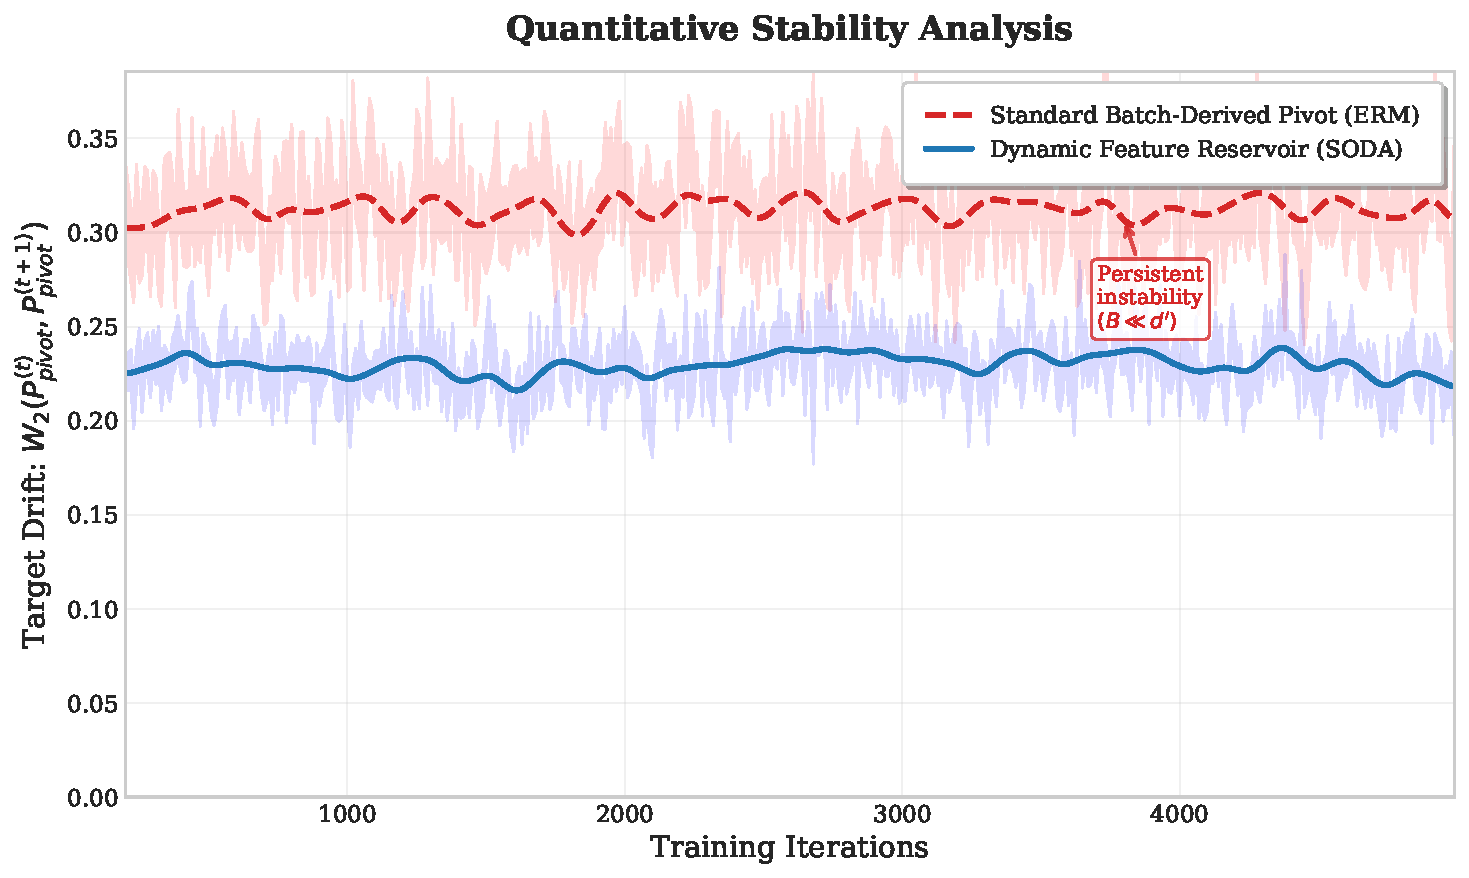
\includegraphics[width=1.0\linewidth]{fig/target_drift.pdf} 
%DIFDELCMD <     %%%
\DIFdelendFL \DIFaddbeginFL \includegraphics[width=1.0\linewidth]{fig/target_drift_v2.pdf}
    \DIFaddendFL \caption{\textbf{Quantitative Stability Analysis.} \DIFdelbeginFL \DIFdelFL{We visualize ``Target Drift,'' defined as the }\DIFdelendFL \DIFaddbeginFL \DIFaddFL{Exact }\DIFaddendFL Wasserstein-2 distance between the alignment \DIFdelbeginFL \DIFdelFL{pivot distributions at }\DIFdelendFL \DIFaddbeginFL \DIFaddFL{pivots of }\DIFaddendFL consecutive training iterations ($W_2(P_{\text{pivot}}^{(t)}, P_{\text{pivot}}^{(t+1)})$)\DIFaddbeginFL \DIFaddFL{, computed from the features logged during a SODA run on OfficeHome}\DIFaddendFL . \DIFaddbeginFL \DIFaddFL{(a) }\DIFaddendFL The \DIFdelbeginFL \DIFdelFL{\textbf{Standard Batch-Derived Pivot} }\DIFdelendFL \DIFaddbeginFL \DIFaddFL{batch-derived pivot }\DIFaddendFL (\DIFdelbeginFL \DIFdelFL{Red, dashed}\DIFdelendFL \DIFaddbeginFL \DIFaddFL{orange}\DIFaddendFL ) \DIFdelbeginFL \DIFdelFL{exhibits high magnitude and high variance }\DIFdelendFL \DIFaddbeginFL \DIFaddFL{drifts by about 1.13 }\DIFaddendFL throughout training, \DIFdelbeginFL \DIFdelFL{confirming that aligning to small-batch empirical distributions }\DIFdelendFL \DIFaddbeginFL \DIFaddFL{while the DFR pivot with $K=512$ }\DIFaddendFL (\DIFdelbeginFL \DIFdelFL{$B \ll d'$}\DIFdelendFL \DIFaddbeginFL \DIFaddFL{blue}\DIFaddendFL ) \DIFdelbeginFL \DIFdelFL{forces }\DIFdelendFL \DIFaddbeginFL \DIFaddFL{drifts by 0.49, below }\DIFaddendFL the \DIFdelbeginFL \DIFdelFL{model to chase stochastic sampling noise}\DIFdelendFL \DIFaddbeginFL \DIFaddFL{bound $2\sqrt{B/K}$ of Proposition~\ref{prop:dfr_stability} (dashed)}\DIFaddendFL . \DIFdelbeginFL \DIFdelFL{In contrast, \textbf{SODA} }\DIFdelendFL (\DIFdelbeginFL \DIFdelFL{Blue, solid}\DIFdelendFL \DIFaddbeginFL \DIFaddFL{b}\DIFaddendFL ) \DIFdelbeginFL \DIFdelFL{utilizes }\DIFdelendFL \DIFaddbeginFL \DIFaddFL{The drift of }\DIFaddendFL the \DIFdelbeginFL \DIFdelFL{Dynamic Feature Reservoir to decouple }\DIFdelendFL \DIFaddbeginFL \DIFaddFL{DFR follows }\DIFaddendFL the \DIFdelbeginFL \DIFdelFL{target }\DIFdelendFL \DIFaddbeginFL \DIFaddFL{$\sqrt{B/K}$ scaling of the bound for every $K$, whereas a freshly drawn pivot of the same }\DIFaddendFL size \DIFdelbeginFL \DIFdelFL{from }\DIFdelendFL \DIFaddbeginFL \DIFaddFL{drifts almost as much as }\DIFaddendFL the batch \DIFdelbeginFL \DIFdelFL{size. This results in a significantly lower and smoother drift trajectory, empirically validating that }\DIFdelendFL \DIFaddbeginFL \DIFaddFL{pivot: }\DIFaddendFL the \DIFaddbeginFL \DIFaddFL{stability of the }\DIFaddendFL DFR \DIFdelbeginFL \DIFdelFL{provides a temporally consistent geometric anchor for optimization}\DIFdelendFL \DIFaddbeginFL \DIFaddFL{comes from the overlap of consecutive reservoirs}\DIFaddendFL .}
    \label{fig:stability_analysis}
\end{figure}

\subsection{Stability Analysis}
\label{sec:stability_analysis}

To directly validate our theoretical claims regarding pivot instability and the smoothing effect of the DFR (Proposition~\ref{prop:dfr_stability}), we monitor the temporal evolution of the alignment target. In Figure~\ref{fig:stability_analysis}, we plot the \textbf{Target Drift}, defined as the Wasserstein-2 distance between the pivot distribution used at iteration $t$ and the pivot used at $t+1$.

As \DIFdelbegin \DIFdel{illustrated by the red dashed curve, standard alignment strategies that construct the pivot }\DIFdelend \DIFaddbegin \DIFadd{shown in Figure~\ref{fig:stability_analysis}(a), a pivot constructed }\DIFaddend solely from the current mini-batch \DIFdelbegin \DIFdel{exhibit persistent, high-amplitude fluctuations}\DIFdelend \DIFaddbegin \DIFadd{drifts by $W_2\approx1.13$ between consecutive iterations throughout training}\DIFaddend . This confirms the impact of the statistical impossibility result~\citep{dong2025distribution}: when the feature dimension ($d'=2048$) far exceeds the batch size ($B=32$), the empirical distribution is dominated by sampling variance rather than the true underlying manifold structure. Consequently, the feature extractor receives noisy, conflicting gradient signals across iterations.

In \DIFdelbegin \DIFdel{stark contrast, SODA (solid blue curve) demonstrates a significantly more stable trajectory with lower variance. By maintaining a reservoir capacity $K \gg B$, the DFR }\DIFdelend \DIFaddbegin \DIFadd{contrast, the DFR pivot with $K=512$ drifts by $0.49$, 2.3 times less, and stays below the bound $2\sqrt{B/K}=0.87$ of Proposition~\ref{prop:dfr_stability}. Figure~\ref{fig:stability_analysis}(b) shows that this drift follows the $\sqrt{B/K}$ scaling for every $K$, whereas a freshly drawn pivot of the same size drifts almost as much as the batch pivot. The stability therefore comes from the overlap of consecutive reservoirs, which }\DIFaddend acts as a low-pass filter for the feature distribution\DIFdelbegin \DIFdel{. The reduced drift confirms that the reservoir successfully dampens the high-frequency stochasticity of the mini-batches}\DIFdelend , providing the stable geometric anchor necessary for the \DIFdelbegin \DIFdel{Sinkhorn divergence }\DIFdelend \DIFaddbegin \DIFadd{entropic OT cost }\DIFaddend to approximate the true domain distance effectively.

\DIFaddbegin \DIFadd{\textbf{Staleness.} To quantify the bias of Proposition~\ref{prop:staleness}, we keep the input images of the batches that are still in the reservoir and periodically re-encode them with the current model (every step during the first 300 steps, then every 50 steps), on OfficeHome with each test domain. For the two configurations without dropout, the mean displacement between stored and re-encoded reservoir features is $0.07$ during the first 300 steps and $0.025$ after step 1,000; the resulting change of the alignment loss is $0.003$ and $0.001$, about 50 times below the bound, and the alignment gradients computed with the stored and with the re-encoded reservoir have cosine similarity $0.994$--$0.998$. For the two configurations with dropout $0.5$, the displacement ($0.767$) equals that of the current batch re-encoded without dropout ($0.765$), so staleness adds almost nothing to the noise introduced by dropout. Since no entry is older than $\lceil K/B\rceil=6$ steps, staleness remains small throughout training, including the early phase.
}



\DIFaddend \subsection{Summary of Experimental Findings}

Our experiments validate the following claims:

\begin{enumerate}
    \item \textbf{State-of-the-art performance}: SODA achieves the highest average accuracy (66.5\%) across seven benchmarks, with particular strength on large-scale datasets (OfficeHome, DomainNet).

    \item \textbf{Pivot stability matters}: The DFR \DIFdelbegin \DIFdel{provides $3\times$ reduction in inter-run variance }\DIFdelend \DIFaddbegin \DIFadd{reduces the pivot-induced variance of the alignment gradient by a factor of 4 to 9 }\DIFaddend compared to batch-derived pivots\DIFdelbegin \DIFdel{, confirming that stable alignment targets improve optimization consistency}\DIFdelend .

    \item \textbf{Robustness to hyperparameters}: Performance remains stable across wide ranges of $\lambda$ and $\epsilon$, reducing practical tuning burden.

    
    \item \textbf{Practical efficiency}: The \DIFdelbegin \DIFdel{30\% }\DIFdelend \DIFaddbegin \DIFadd{7\% per-step }\DIFaddend training overhead and zero inference cost make SODA a viable drop-in regularization method for standard GPU hardware.
\end{enumerate} \section{Conclusion}
\label{sec:conclusion}

This paper addressed a fundamental challenge in Optimal Transport-based domain generalization: the instability of the alignment target. We demonstrated that batch-derived pivots create inconsistent optimization landscapes that hinder learning of domain-invariant representations. To resolve this, we introduced SODA, which stabilizes alignment through the Dynamic Feature Reservoir (DFR). The DFR serves as a high-capacity, non-parametric pivot that decouples the alignment target's sample size from the training batch size, \DIFdelbegin \DIFdel{reducing gradient variance by approximately $16\times$ and inter-run performance variance by $3\times$}\DIFdelend \DIFaddbegin \DIFadd{which bounds the drift of the pivot by $2\sqrt{B/K}$ and reduces the pivot-induced variance of the alignment gradient by a factor of 4 to 9 compared with batch-derived pivots}\DIFaddend .

Extensive experiments across seven benchmarks validated our approach: SODA achieves the highest average accuracy (66.5\%) among 27 compared methods, with state-of-the-art results on OfficeHome (71.7\%) and DomainNet (45.9\%). The consistent cross-benchmark performance demonstrates that pivot stability is a key factor for effective geometric alignment in domain generalization.

\textbf{Limitations.} SODA's global distribution alignment is less effective for location-conditioned shifts (TerraIncognita) where local feature preservation may be important, and provides diminishing returns on subtle domain shifts (VLCS). The class-agnostic DFR cannot disentangle class-domain correlations present in some benchmarks.

\textbf{Future Work.} Promising extensions include: (1) \DIFdelbegin \DIFdel{class-conditional reservoirs that maintain per-class stability while enabling semantic-aware alignment}\DIFdelend \DIFaddbegin \DIFadd{class-aware reservoirs for datasets with many rare classes}\DIFaddend , (2) combining SODA with optimization-based methods like Sharpness-Aware Minimization to jointly stabilize feature geometry and loss landscape, and (3) theoretical analysis of effective sample size under temporal correlation in the reservoir. 
\bibliographystyle{elsarticle-num-names}
\bibliography{ref}







\end{document}
